% This is the file main.tex
\usepackage{group4}
\begin{document}
	
	% (The following generates the slides) 
	%---------------------------------------------------------------------------------------------------------------------------------------------------------------------------------------
\mode<presentation>{
	\begin{frame}
	\titlepage
\end{frame}


	\section*{Outline}
	\begin{frame}{Outline}
		\tableofcontents
	\end{frame}
	
\section{Initial Plots}

  
  	\begin{frame}{Second differences with and without seasonal adjustments}
  		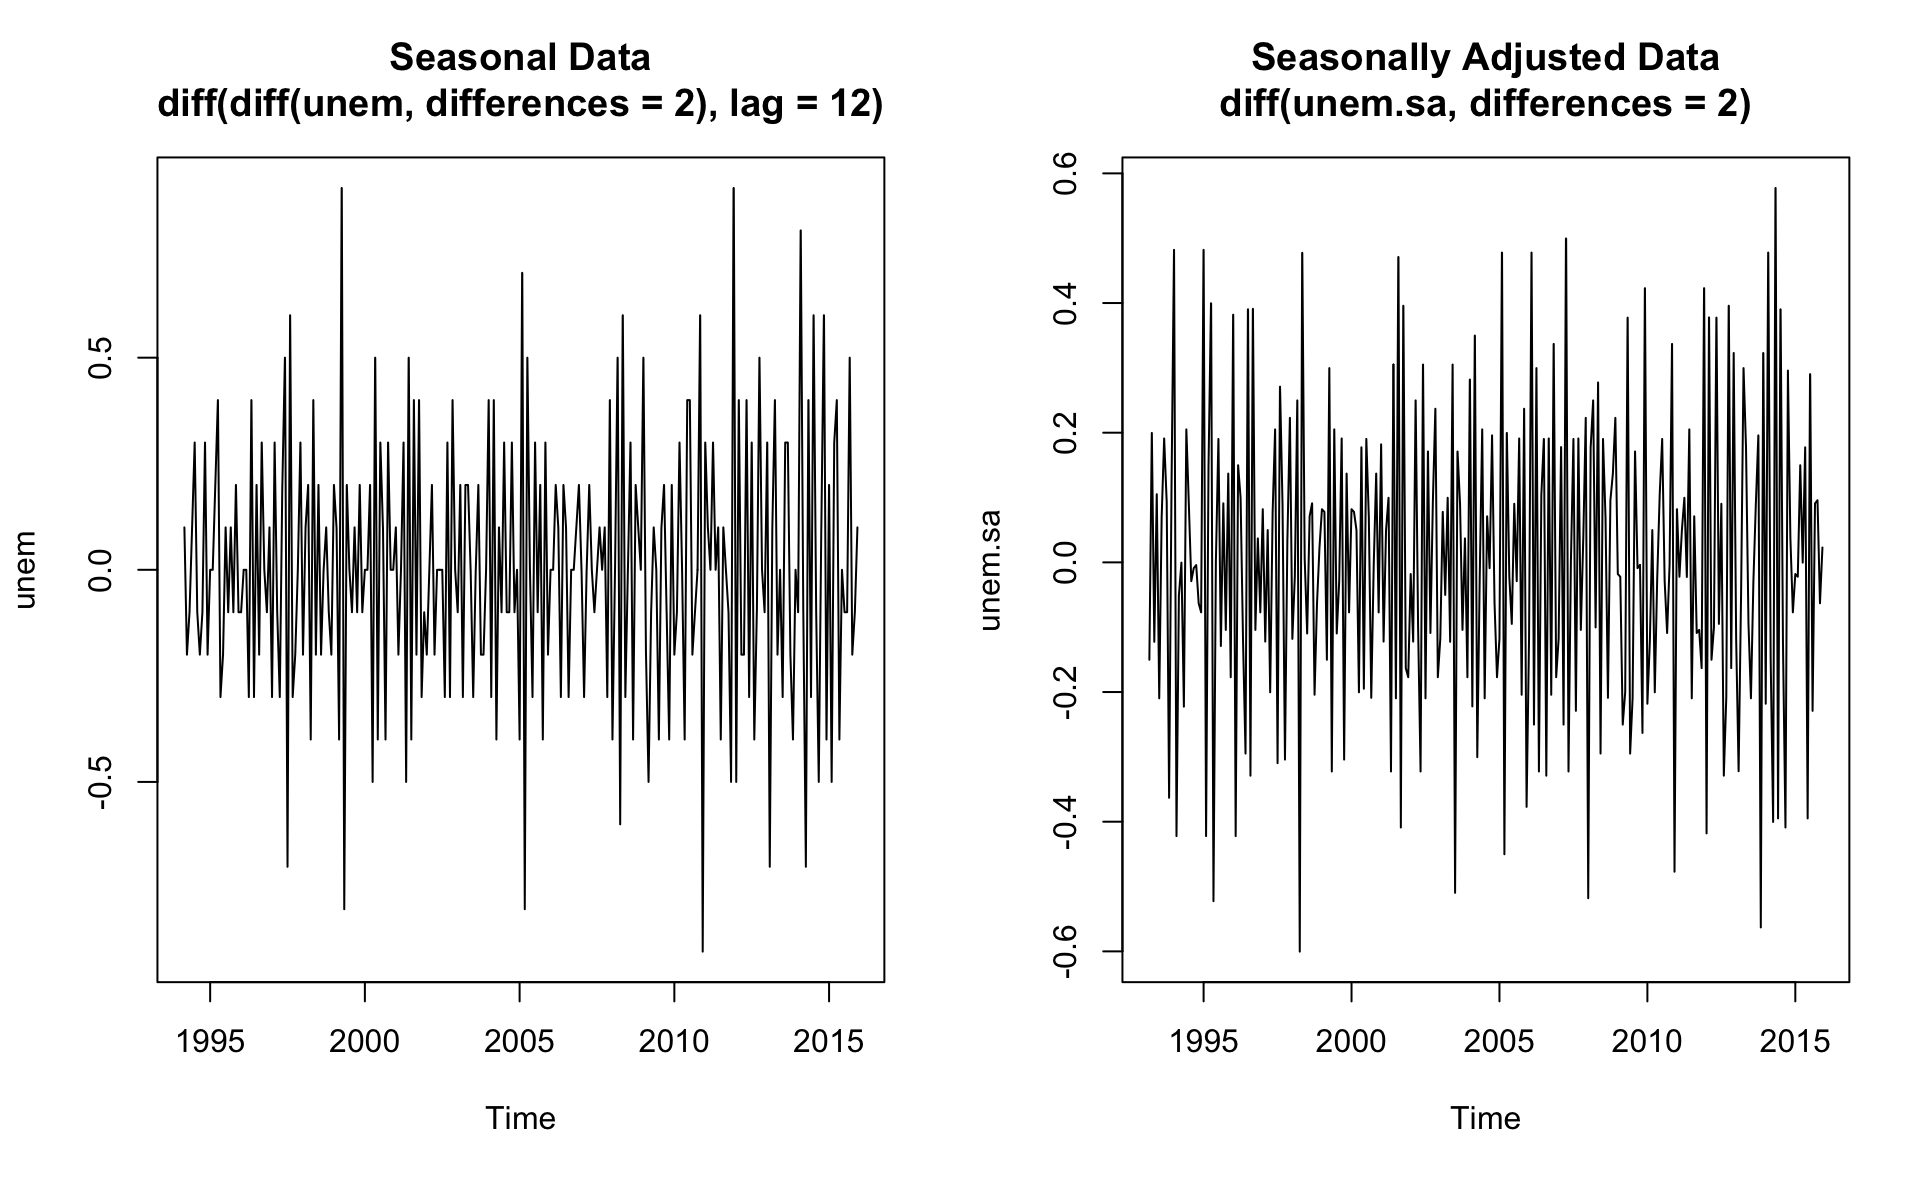
\includegraphics[width=.9\linewidth]{images/stationarity}
  	\end{frame}
  	
  	  
  	  \subsection{ACF \& PACF}
  	  \begin{frame}{ACF \& PACF Plots}
  	  	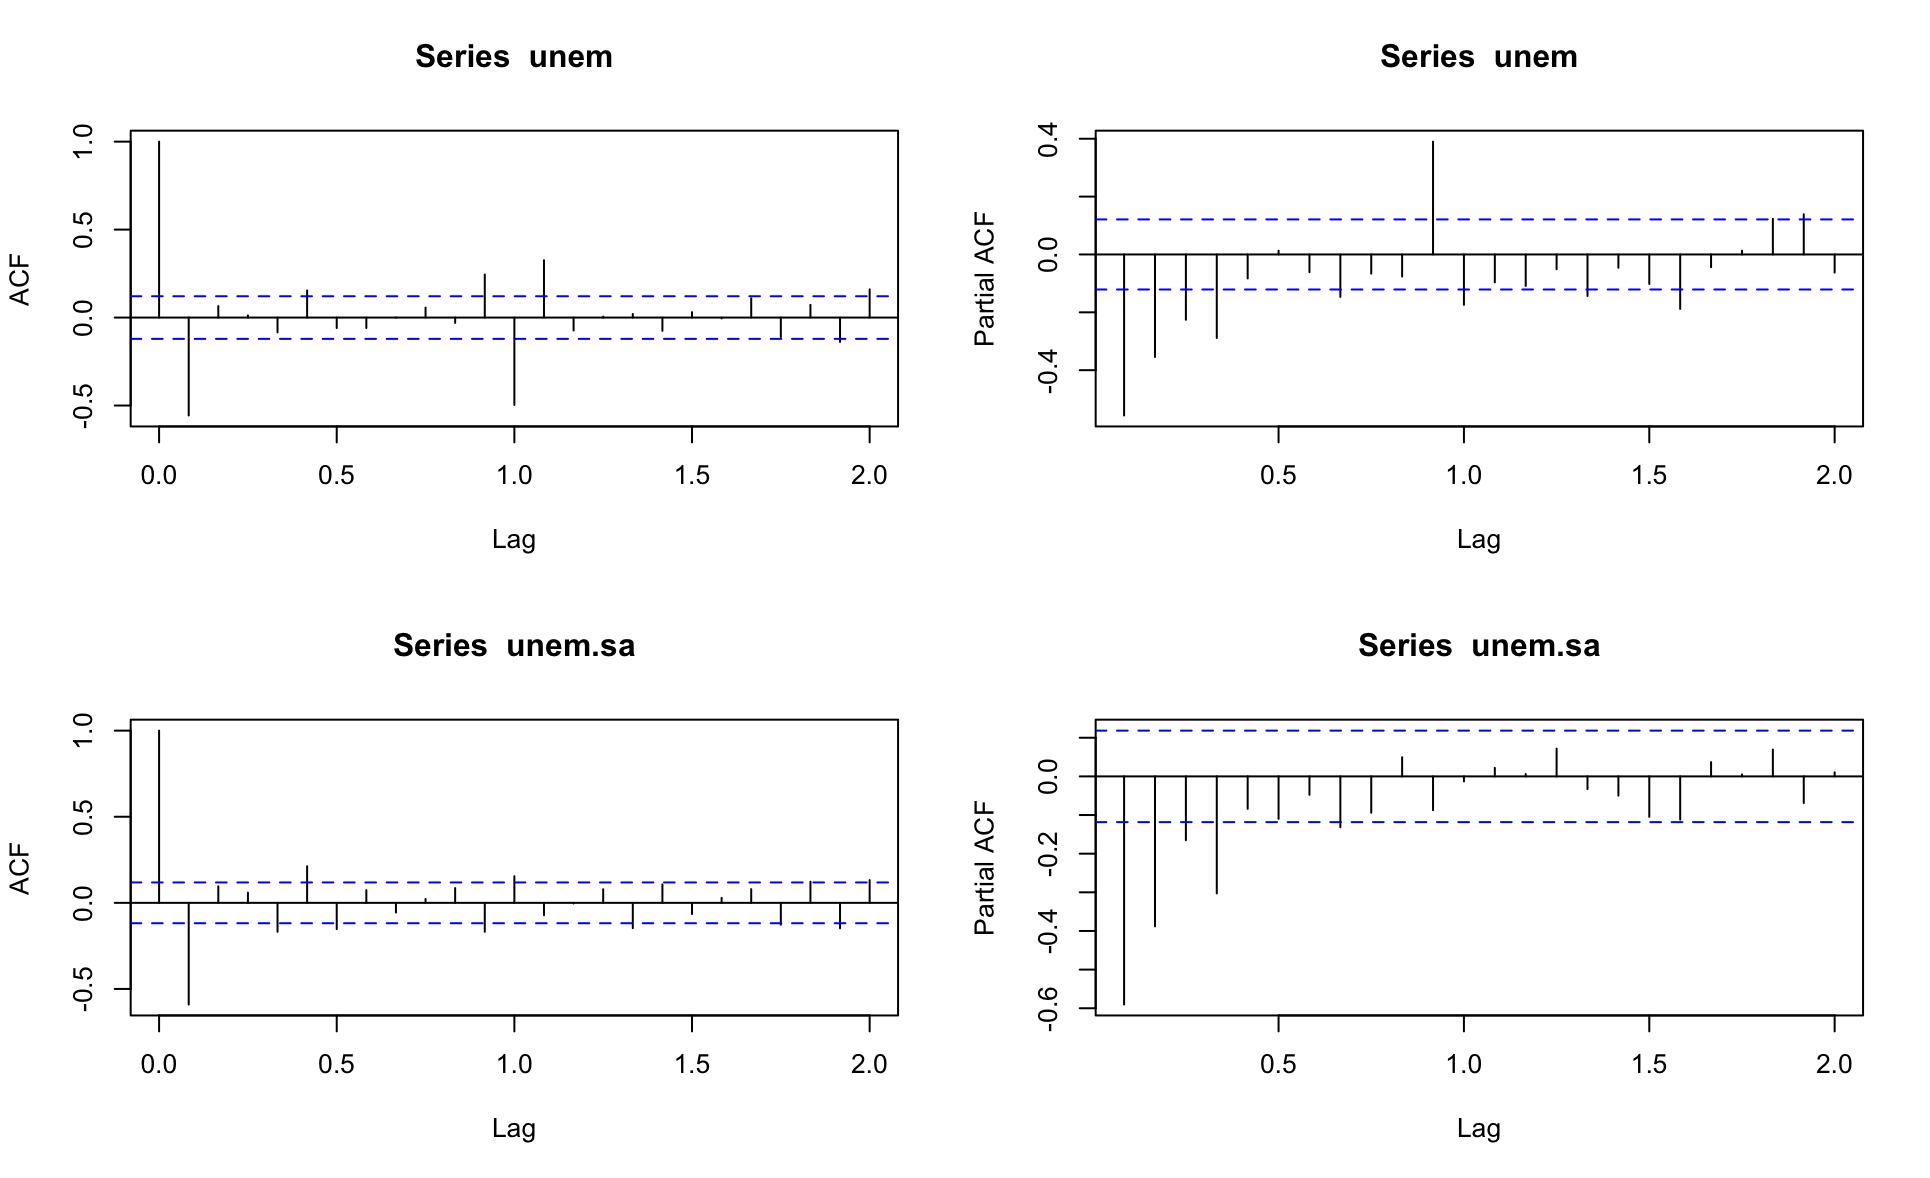
\includegraphics[width=.9\linewidth]{images/acfpacf}
  	  \end{frame}
 
     \subsection{Overview}
     \begin{frame}{Models Considered}
     	% latex table generated in R 3.2.4 by xtable 1.8-2 package
     	% Thu Jul  7 16:13:24 2016
     	\begin{table}[H]
     		\centering
     		\caption{Model Summaries}
     		\begin{tabular}{llccccc}
     			\hline
     			\textbf{\#}& \textbf{Data}  & \textbf{Order} & \textbf{Seasonal} & \textbf{XRegs} & \textbf{AIC} & \textbf{BIC} \\
     			&&&\textbf{Order}&&&\\ 
     			\hline
     			1 & Unem  & 0,2,1 & 1,1,0 & N & -2.27 & -3.23 \\ 
     			2 & Unem  & 0,2,1 & 3,1,0 & N & -2.44 & -3.37 \\ 
     			3 & Unem  & 4,2,1 & 3,1,0 & N & -2.44 & -3.32 \\ 
     			4 & Unem.sa & 0,2,1 & 1,0,0 & N & -2.61 & -3.58 \\ 
     			5 & Unem.sa  & 1,2,1 &  & N & -2.63 & -3.60 \\ 
     			6 & Unem.sa & 0,2,1 & 1,0,0 & Y & -2.58 & -3.49 \\ 
     			7 & Unem.sa  & 1,2,1 &  & Y & -2.60 & -3.49 \\ 
     			\hline
     		\end{tabular}
     		\label{tab:models}
     	\end{table}
     \end{frame}
     %-----------------------------------------------------------------------------------------
     
     \subsection{Seasonal Models}
     %-----------------------------------------------------------------------------------------
     \begin{frame}{Model 1: SARIMA\((0,2,1) \times (1,1,0)_{12}\)}
     	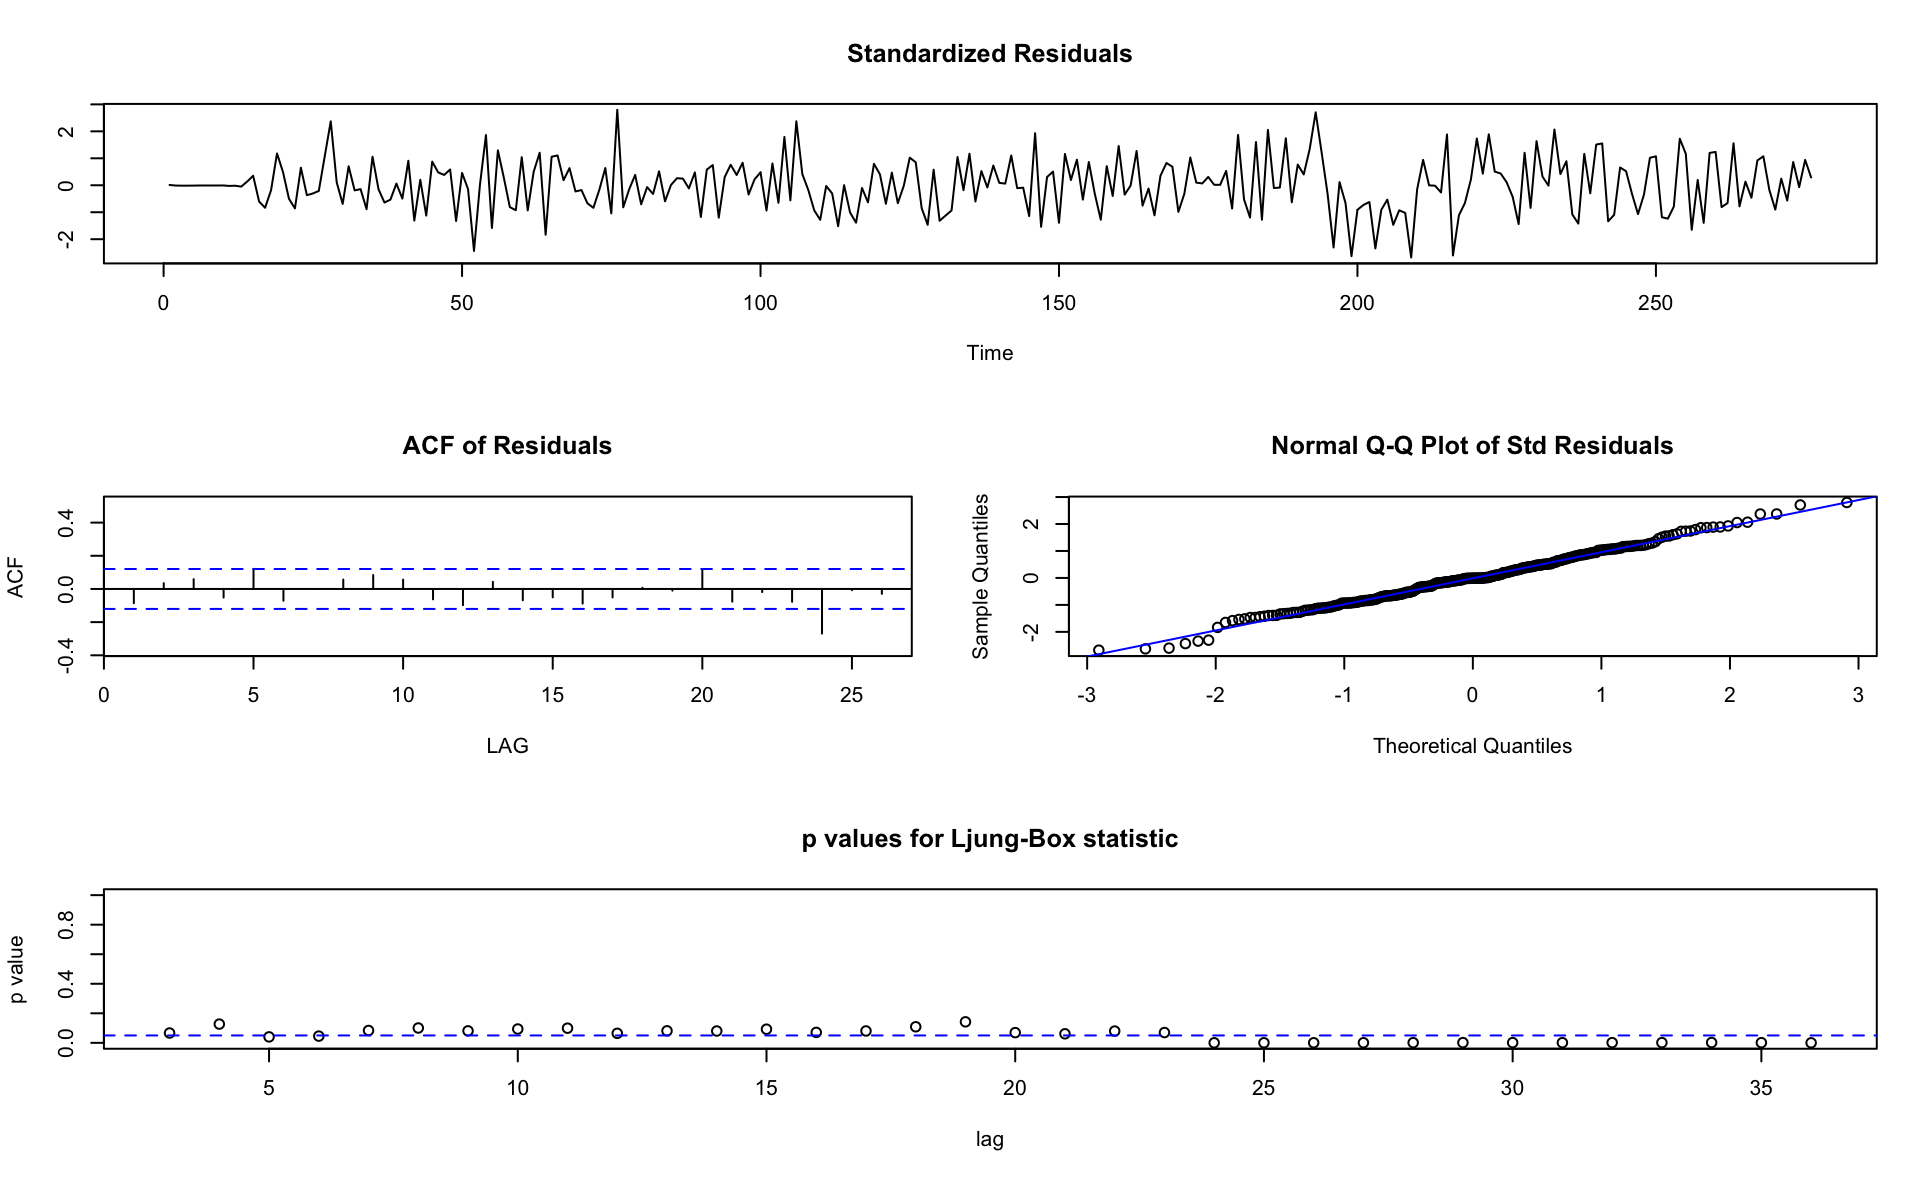
\includegraphics[width=\linewidth]{images/seasonalmodel1}
     \end{frame}
     
     %-----------------------------------------------------------------------------------------
     
     \begin{frame}{Model 2: SARIMA\((0,2,1) \times (3,1,0)_{12}\)}
     	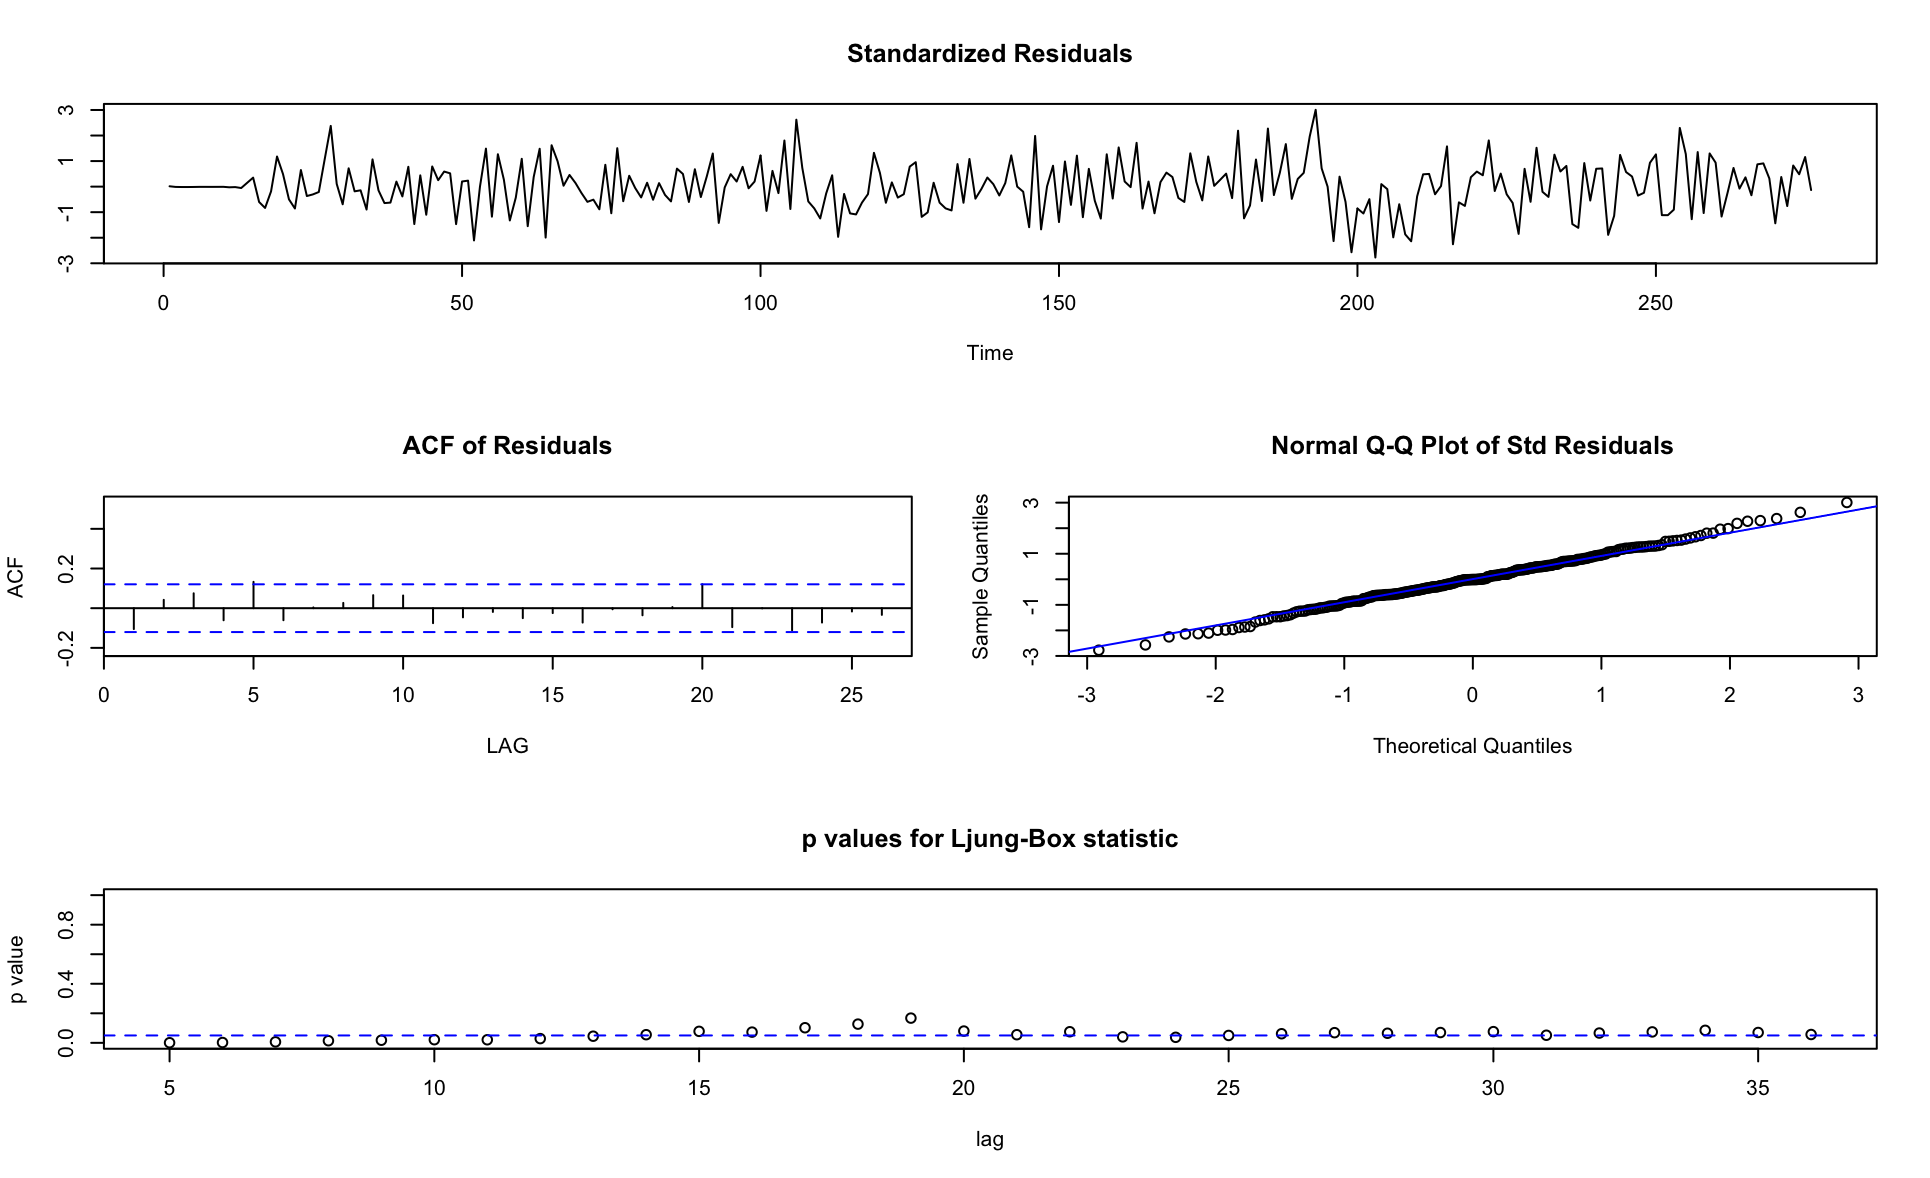
\includegraphics[width=\linewidth]{images/seasonalmodel2}
     \end{frame}  
     
     %-----------------------------------------------------------------------------------------
     
     \begin{frame}{Model 3: SARIMA\((4, 2, 1) \times (3,1,0)_{12}\)}
     	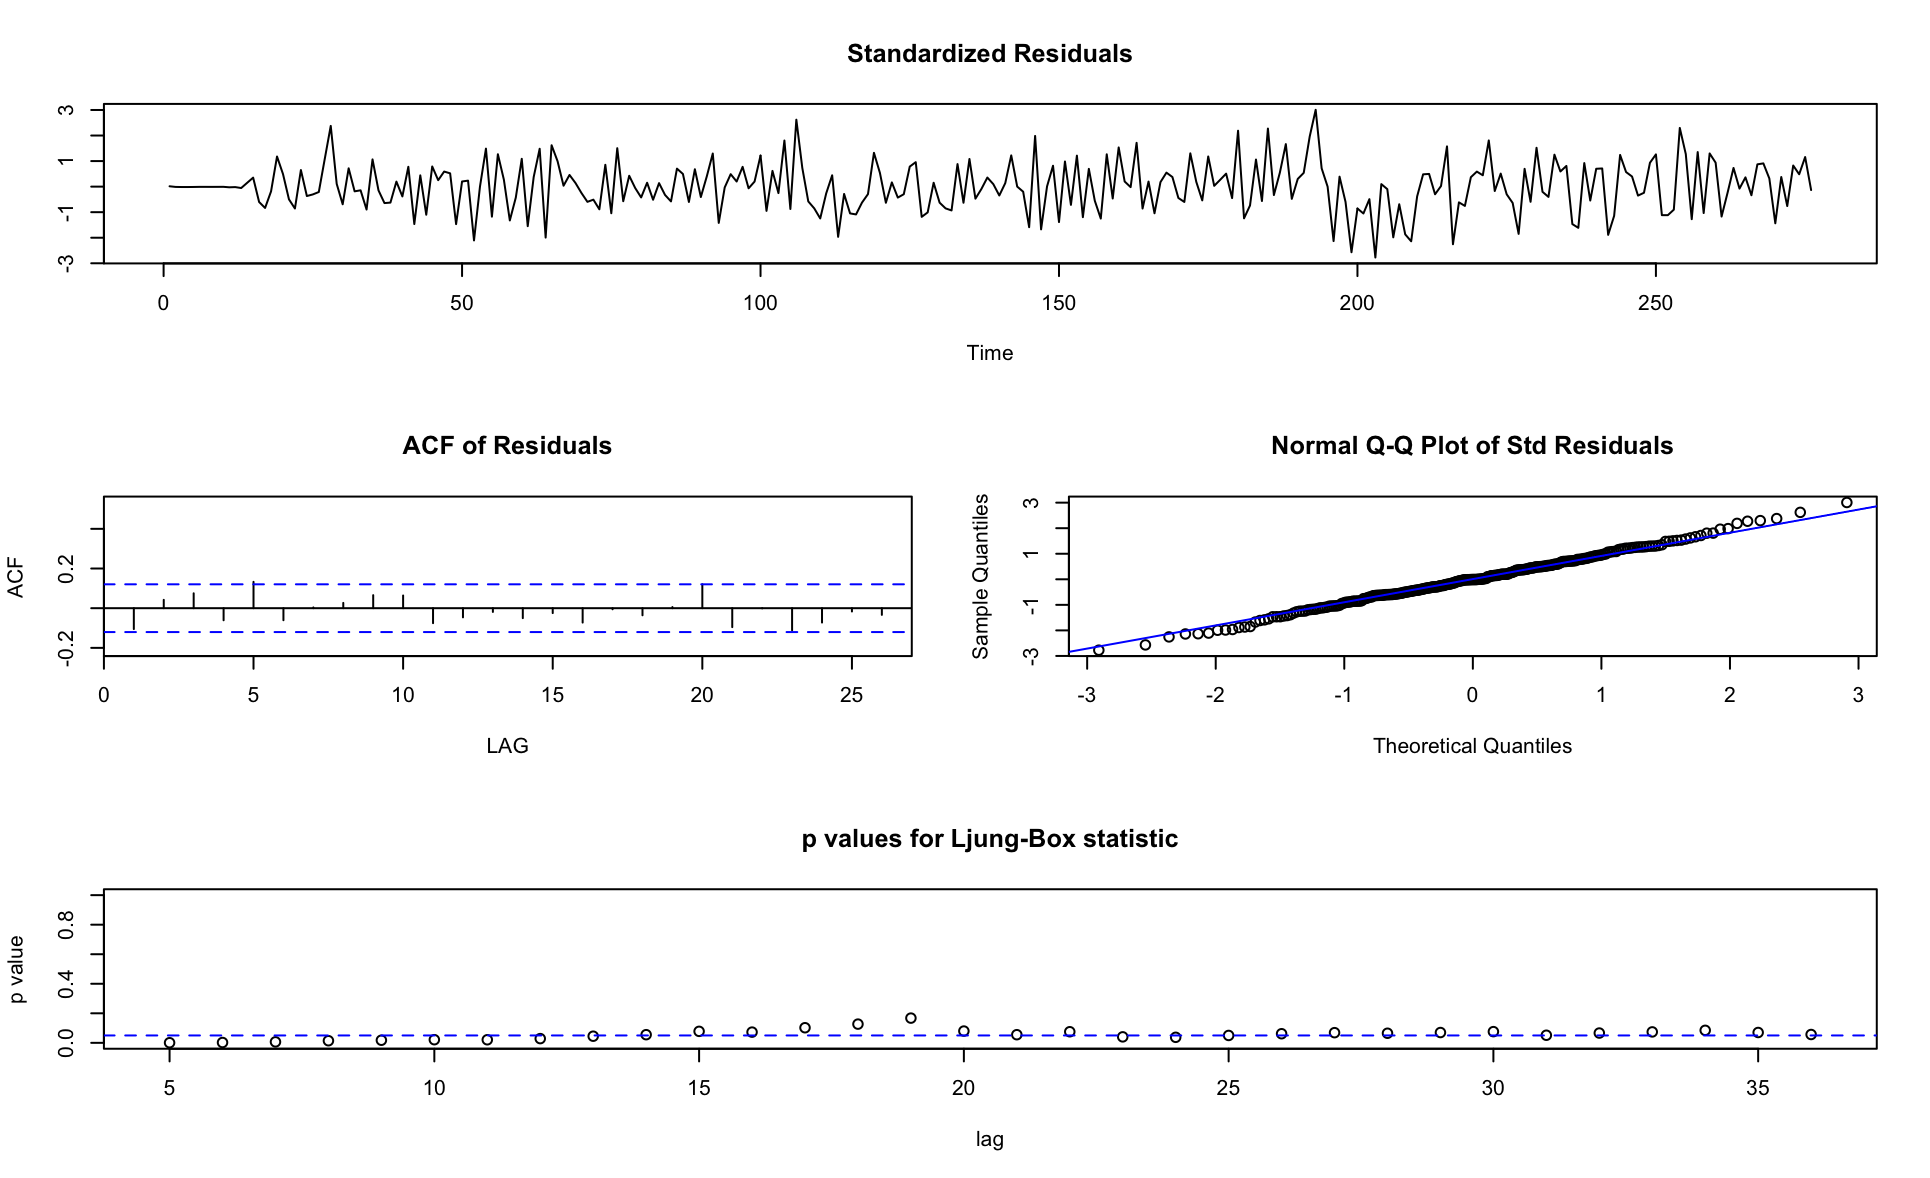
\includegraphics[width=\linewidth]{images/seasonalmodel3}
     \end{frame}  
     %-----------------------------------------------------------------------------------------  
     
     \subsection{Seasonally Adjusted Models}
     %-----------------------------------------------------------------------------------------  
     \begin{frame}{Model 4: SARIMA\((0,2,1) \times (1,0,0)_{12}\)}
     	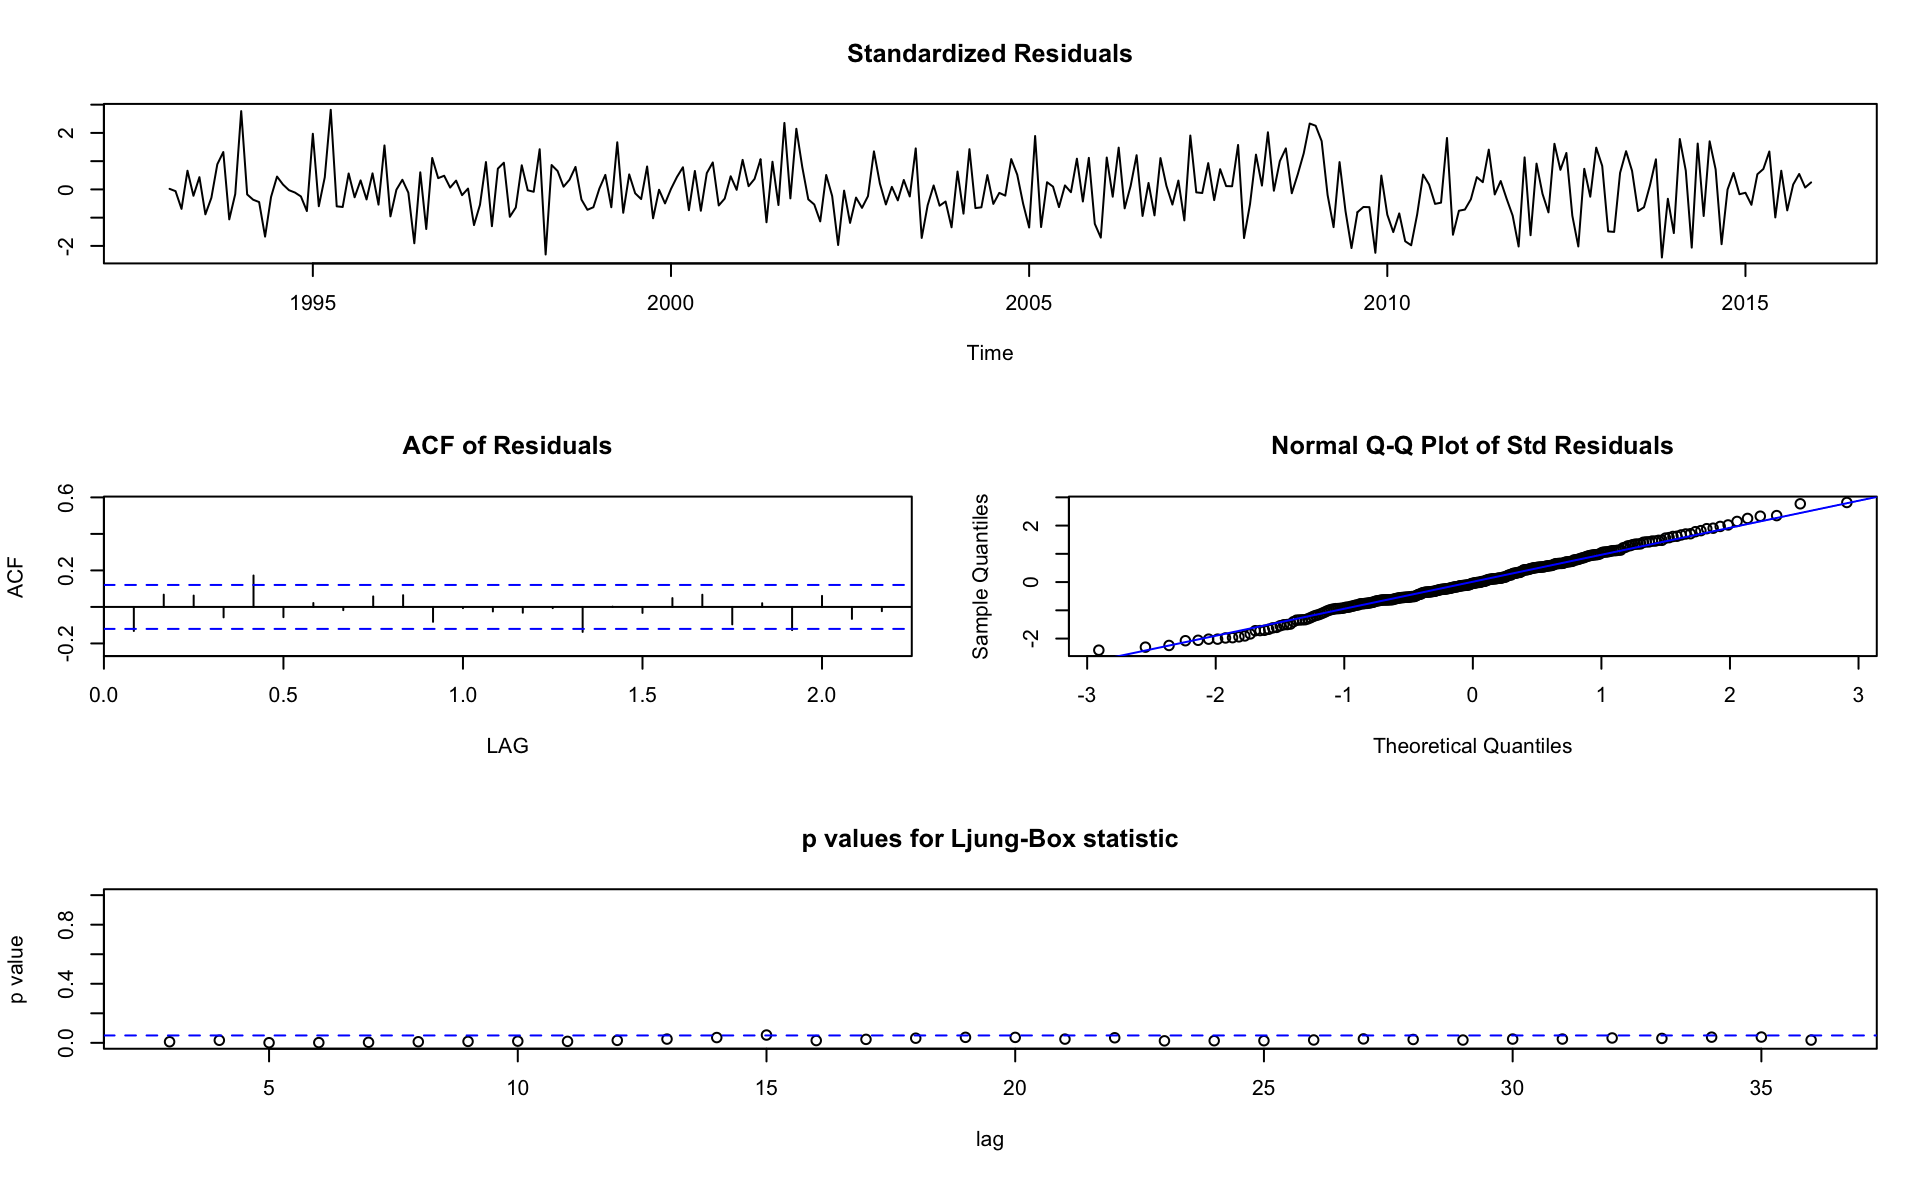
\includegraphics[width=\linewidth]{images/seasonallyadjustedmodel4}
     \end{frame}
     
     %-----------------------------------------------------------------------------------------
     
     \begin{frame}{Model 5: ARIMA\((1,2,1)\)}
     	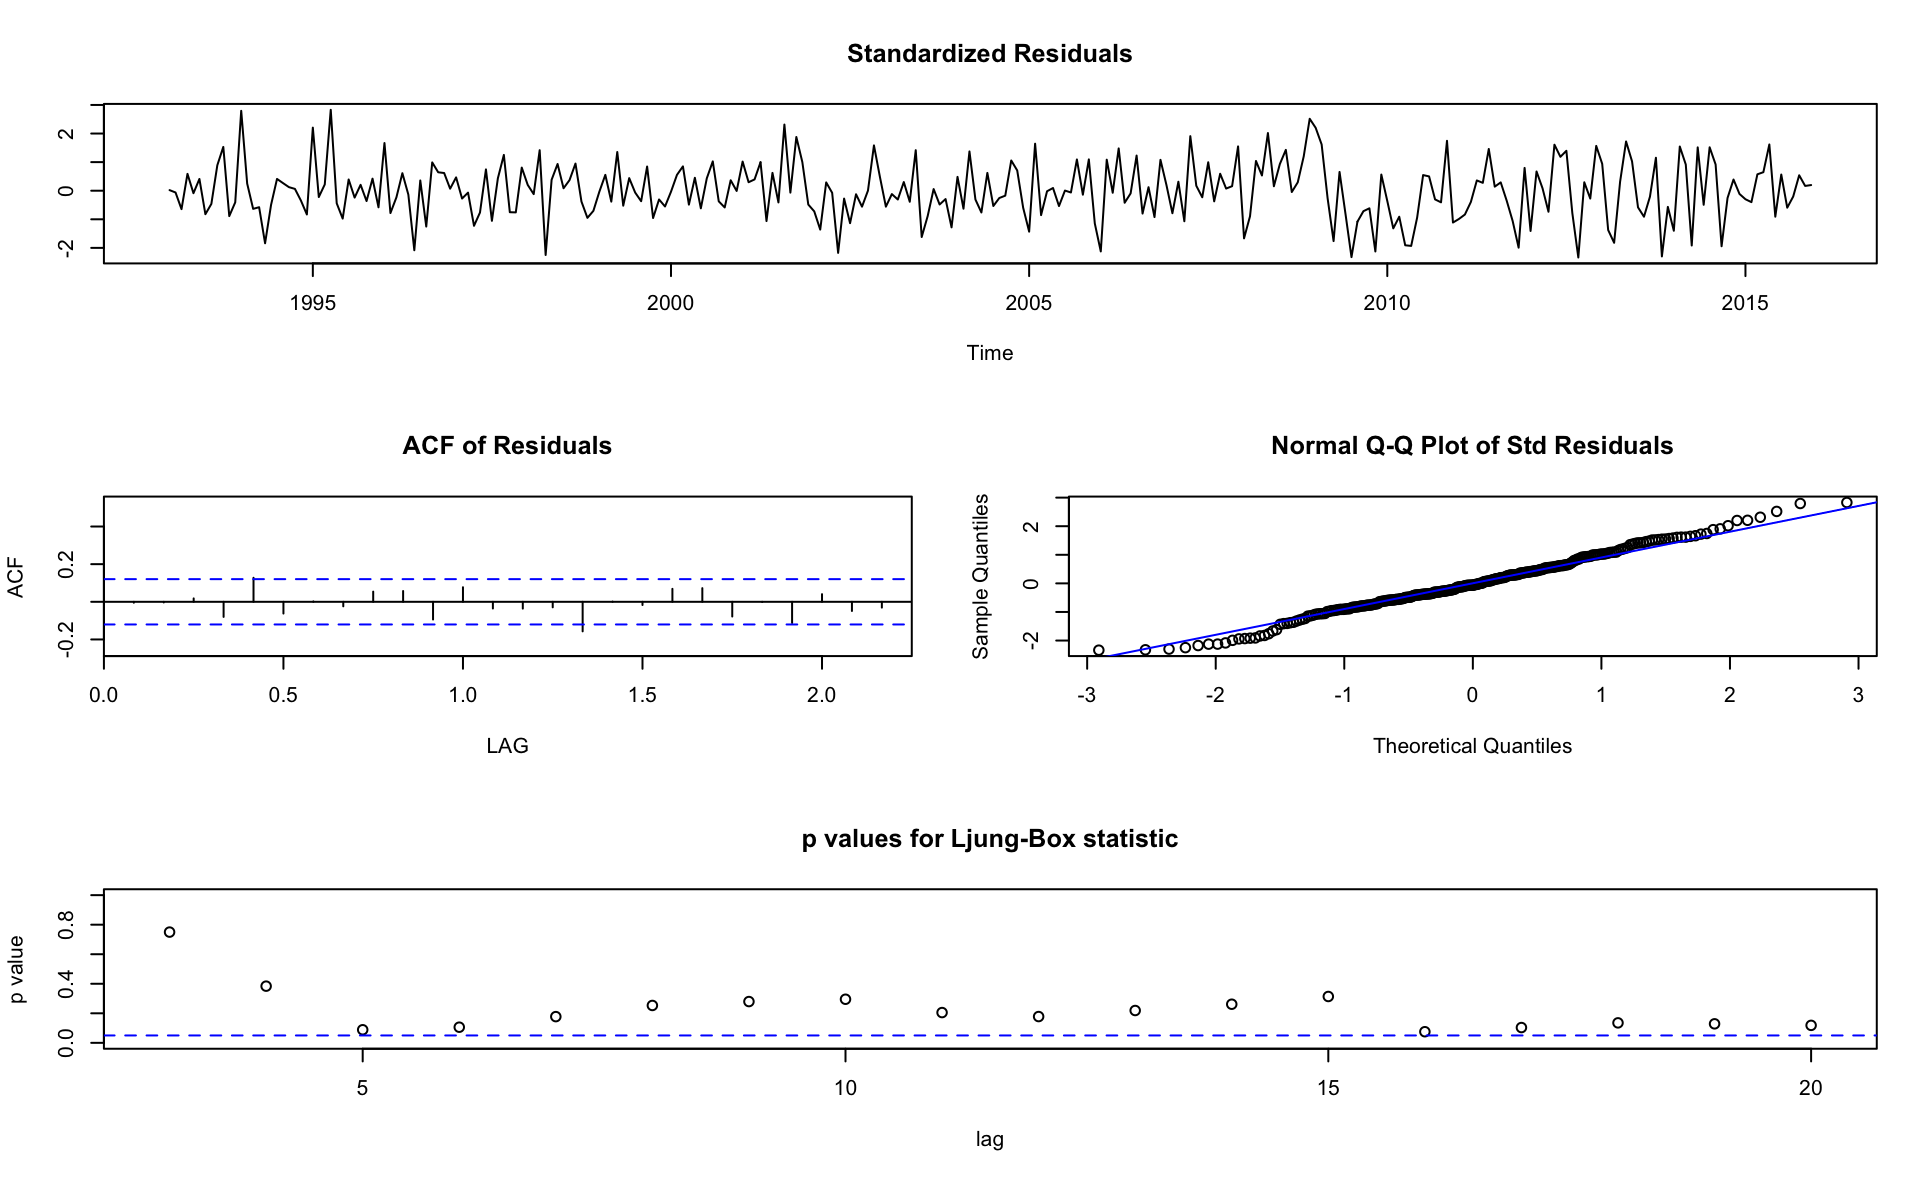
\includegraphics[width=\linewidth]{images/seasonallyadjustedmodel5}
     \end{frame}
     
     %-----------------------------------------------------------------------------------------
     
     \begin{frame}{Model 6: SARIMA\((0,2,1) \times (1,0,0)_{12}\) with Regressors}
     	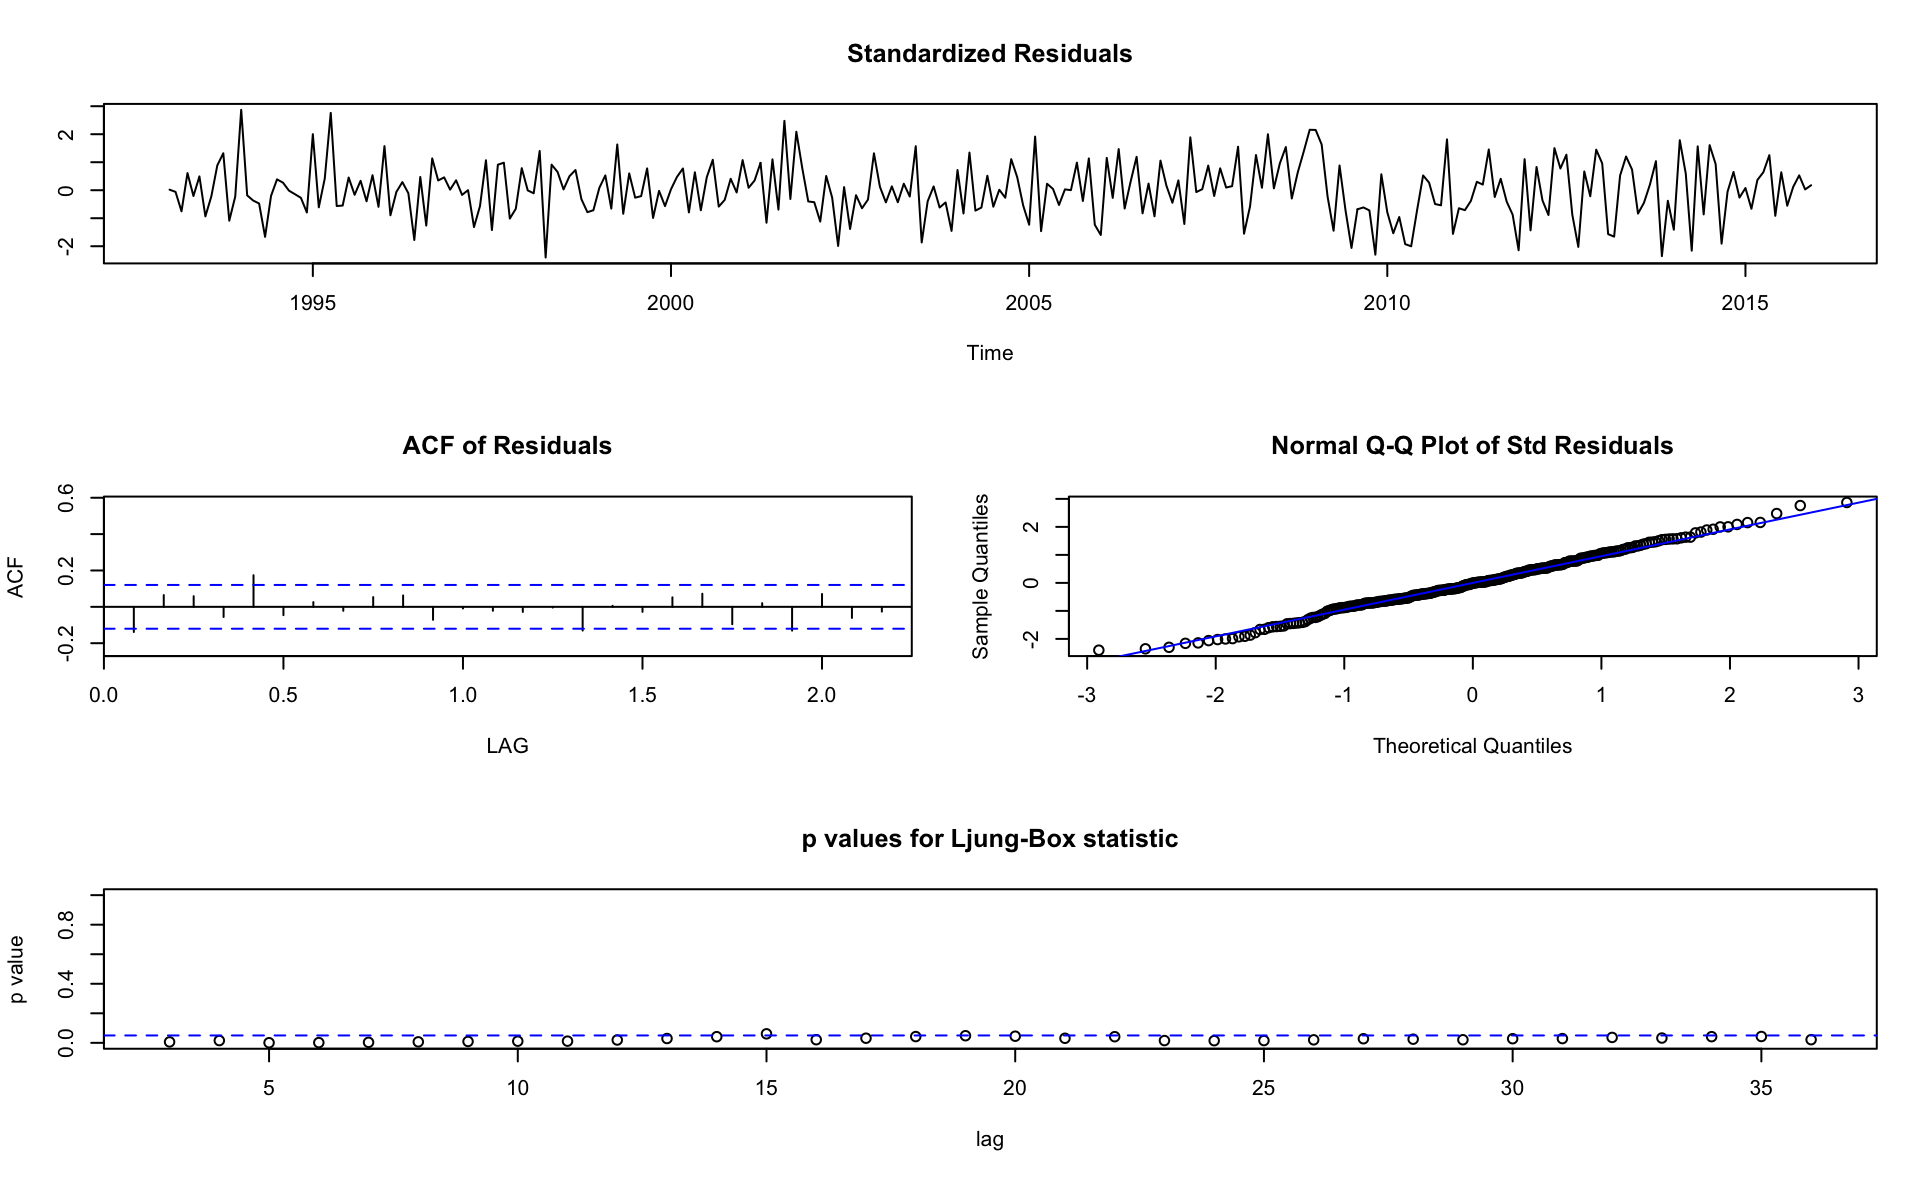
\includegraphics[width=\linewidth]{images/seasonallyadjustedmodel6}
     \end{frame}
     
     %-----------------------------------------------------------------------------------------
     
     \begin{frame}{Model 7: ARIMA\((1,2,1)\) with Regressors}
     	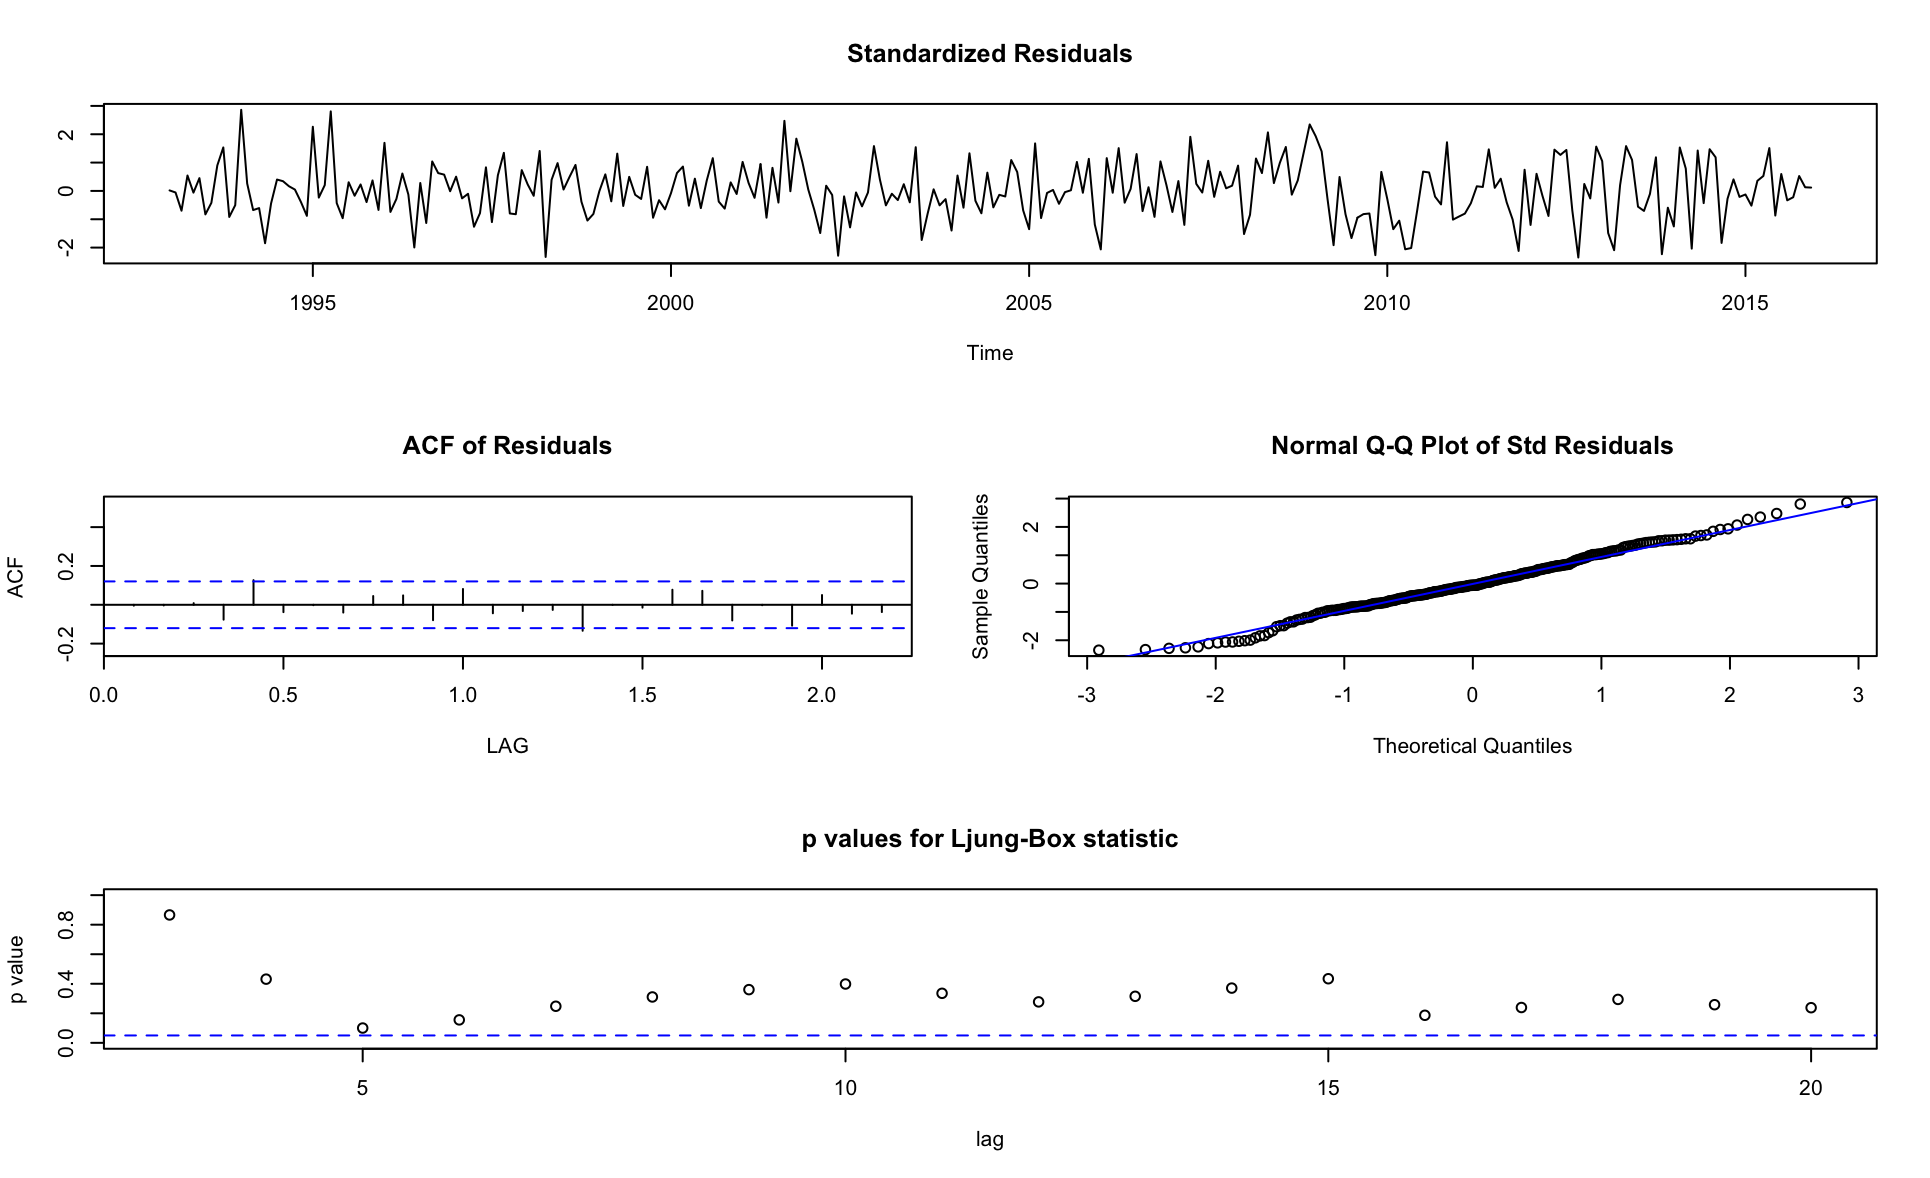
\includegraphics[width=\linewidth]{images/seasonallyadjustedmodel7}
     \end{frame}  
}	
	%--------------------------------------------------------------------------------------------------------------------------------------------------------------------------------------	

% The following generates the write-up
%--------------------------------------------------------------------------------------------------------------------------------------------------------------------------------------	

	
	\mode<article>{
		\title[Unemployment Trends] % (optional, use only with long paper titles)
		{\Huge US Unemployment Trends}
		\subtitle{\huge Initial Model Selection \vspace*{1 cm}}
		\subtitle{\LARGE Group 4}
		
		\date[STAT 626] %(optional, should be abbreviation of conference name)
		{\Large STAT 626: Time Series Analysis}
		% - Either use conference name or its abbreviation.
		% - Not really informative to the audience, more for people (including
		%   yourself) who are reading the slides online
		
		\author[Group 4]{\large Joseph Blubaugh \and Sean Roberson \and Akarshan Puri \and 
			Alison Shelton \and Travis Lilley \and Bo Pang \vspace*{.5 cm}}
		
		\institute[Texas A\&M] % (optional, but mostly needed)
		{Texas A\&M \newline College Station, Texas}
		% - Use the \inst command only if there are several affiliations.
		% - Keep it simple, no one is interested in your street address.

		\pagestyle{fancy}

	\lhead{Group 4}
\chead{}
\rhead{\bfseries US Unemployment Trends} 
\lfoot{}
\cfoot{\thepage}
\rfoot{} 	
		
		\newgeometry{margin=2in}
		\maketitle
		\restoregeometry

		\newpage


		
		
		\subsection*{Introduction}
		
		Unemployment has been a topic of concern throughout the United States in recent years.  Graduate and Undergraduate college students alike are concerned over their employment prospects, wondering if their degrees will be enough to gain them a job after graduation.  In these times of economic uncertainty, obtaining an income generating position is not the guarantee it has seemed to be in generations past. Therefore, the purpose of our project is to examine trends in unemployment in the United States, focusing  on the years from 1992 to 2015, with a goal of forecasting into late 2016 and beyond.  \newline
		
		The unemployment data being examined was obtained from the non-seasonaly adjusted, monthly, Civilian Unemployment Rate Series (UNRATENSA), published by the Bureau of Labor Statistics (BLS).  This series includes unemployment figures from January of 1948 to  May of 2016 \citep{blsref}.  The response variable being analyzed is the unemployment rate defined as the percentage of the labor force that is unemployed.  In defining this variable, the BLS restricts this to, ``people 16 years of age and older, who currently reside in 1 of the 50 states or the District of Columbia, who do not reside in institutions (e.g., penal and mental facilities, homes for the aged), and who are not on active duty in the Armed Forces''. \newline
		
		As a first step, the data was plotted over time to identify any obvious patterns visually, considering both seasonlly adjusted and non-seasonlly adjusted versions of the unemployment rate, see Figure \ref{fig:unemployment}.  The time span included in the study encompases the presidential terms of Bill Clinton, George W. Bush, and Barack Obama, each serving eight years in office.  Initial graphs of the data seem to indicate that, in general, unemployment spiked at the begining of each president's term and fell gradually over the time he was in office. There are also two noticeable spikes the represent that recessions of 2001 and 2008, respectively.  The 2008 recession also follows the burst of a housing market bubble.  These are all potential explanatory variables that will be explored in further analysis.
		\begin{figure}[H]
			\centering
			\caption{Plot of the original data}
			\label{fig:unemployment}
			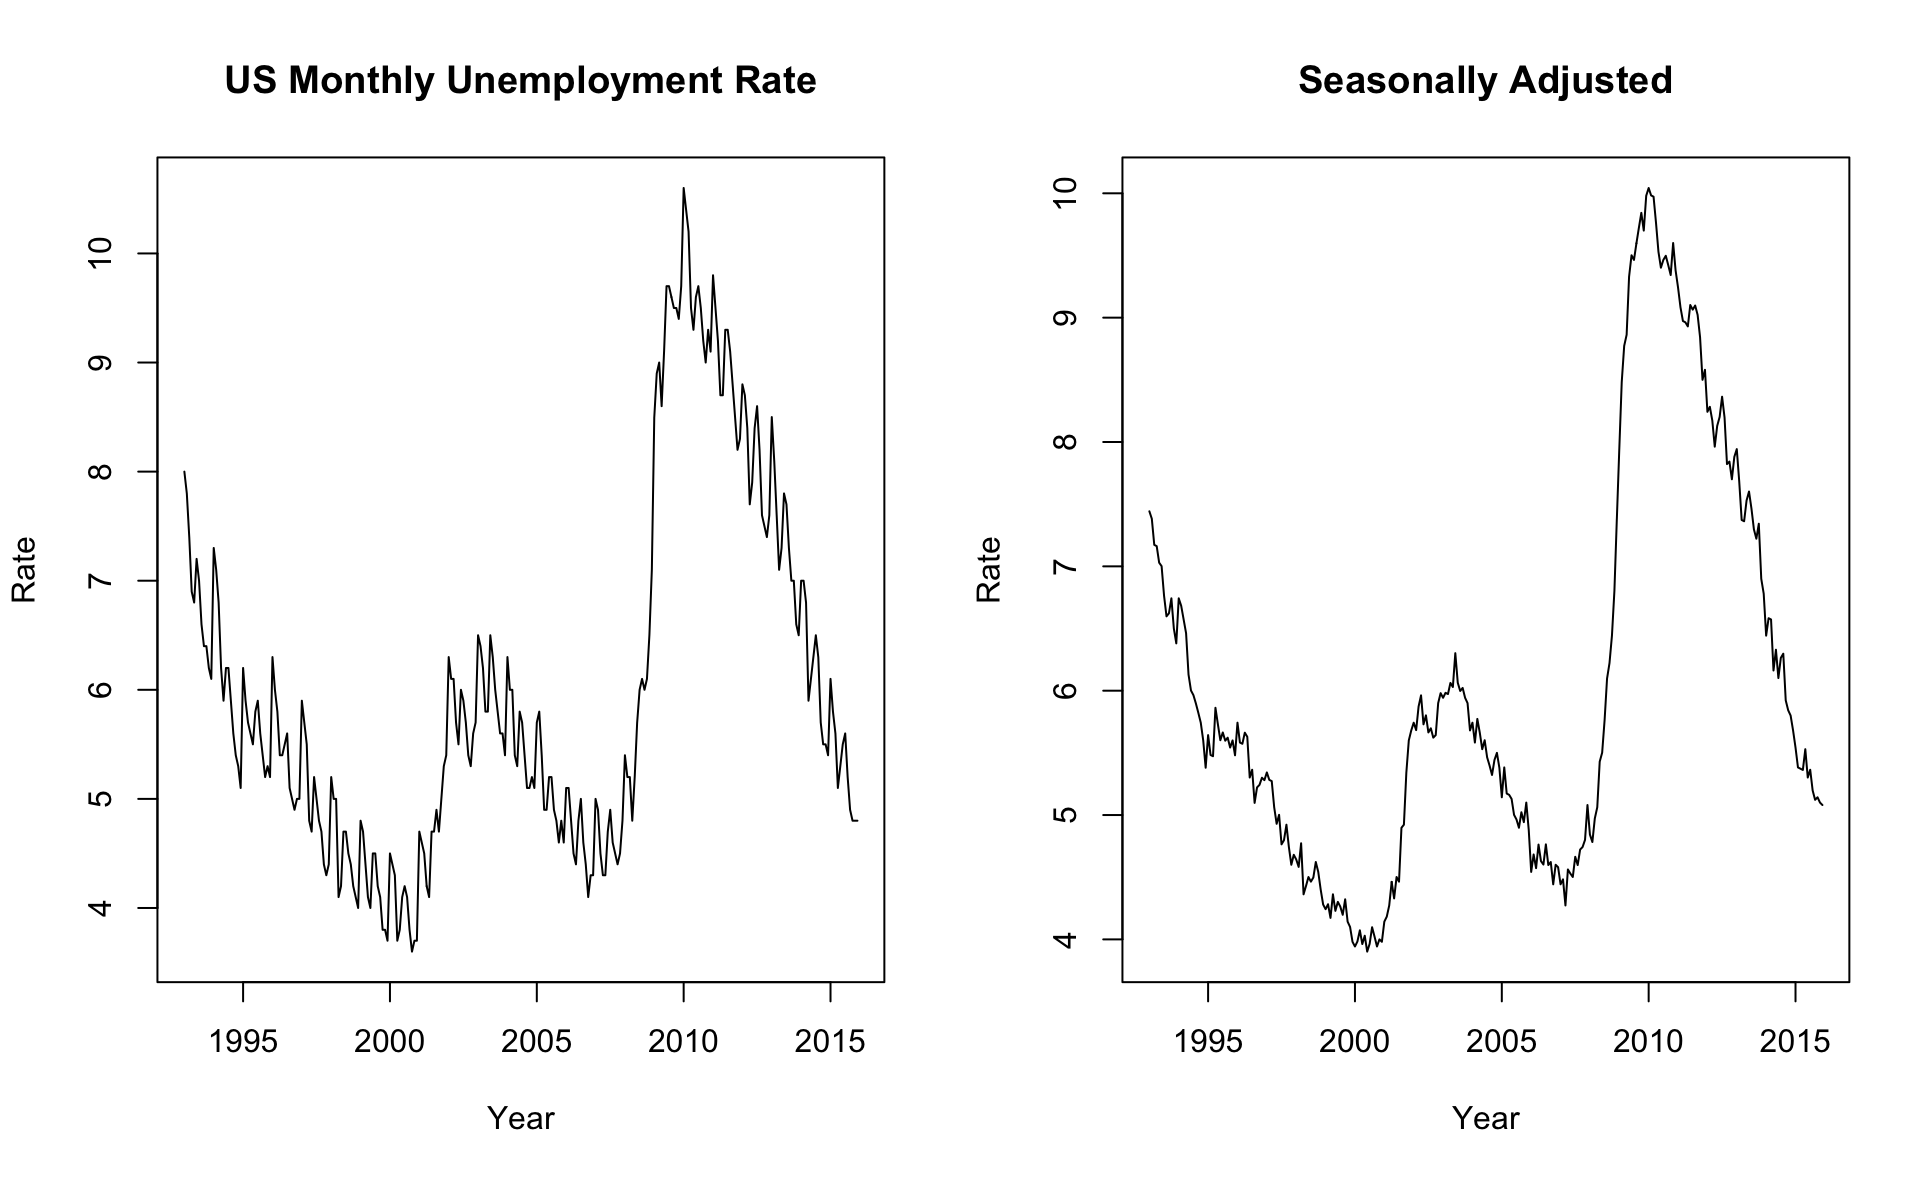
\includegraphics[width=.7\textwidth]{images/Unemployment}
		\end{figure}
		
		\subsection*{Stationarity}
						
			After the initial exploration of the time series graphs, the team has chosen to focus on building priliminary models which will serve as the foundation of further analysis. In looking at the inital plots, it appears that the series could benefit from detrending. As such, one of the primary goals has been to transform the data to stationarity. \newline
			
			An Augmented Dickey-Fuller (ADF) test for stationarity was conducted to verify the nonstationarity of the unemployment data.  The ADF test tests the null hypothesis that the time series data has a unit root against the alternative that the data are stationary \citep{shumway2010time}. For the non-seasonlly adjusted data the Dickey-Fuller test statistic was -1.4266, with a lag order of 6, and a p-value of 0.8176. Additionally, the seasonally adjusted data had a Dickey-Fuller test statistic of -2.1377, also with a lag order of 6, and a p-value of 0.518. The high p-values suggest that we do not have a stationary model with just the raw unemployment data, whether or not the data are seasonally adjusted.\newline
			
		 The first and second differences of the unemployment data were plotted for both the seasonal and seasonally adjusted unemployment data, see Figures \ref{fig:firstdiff} and \ref{fig:secdiff}. Both the first and second differences appear considerably more stationary when compared to the original data. The associated ADF test results are given in Table \ref{tab:ADF}. Based on the p-values, there is significant evidence of stationarity with each of the 4 differenced models. The consensus in the group was to continue the model building using second differences.
		 
	
		 \begin{figure}[H]
							\centering
							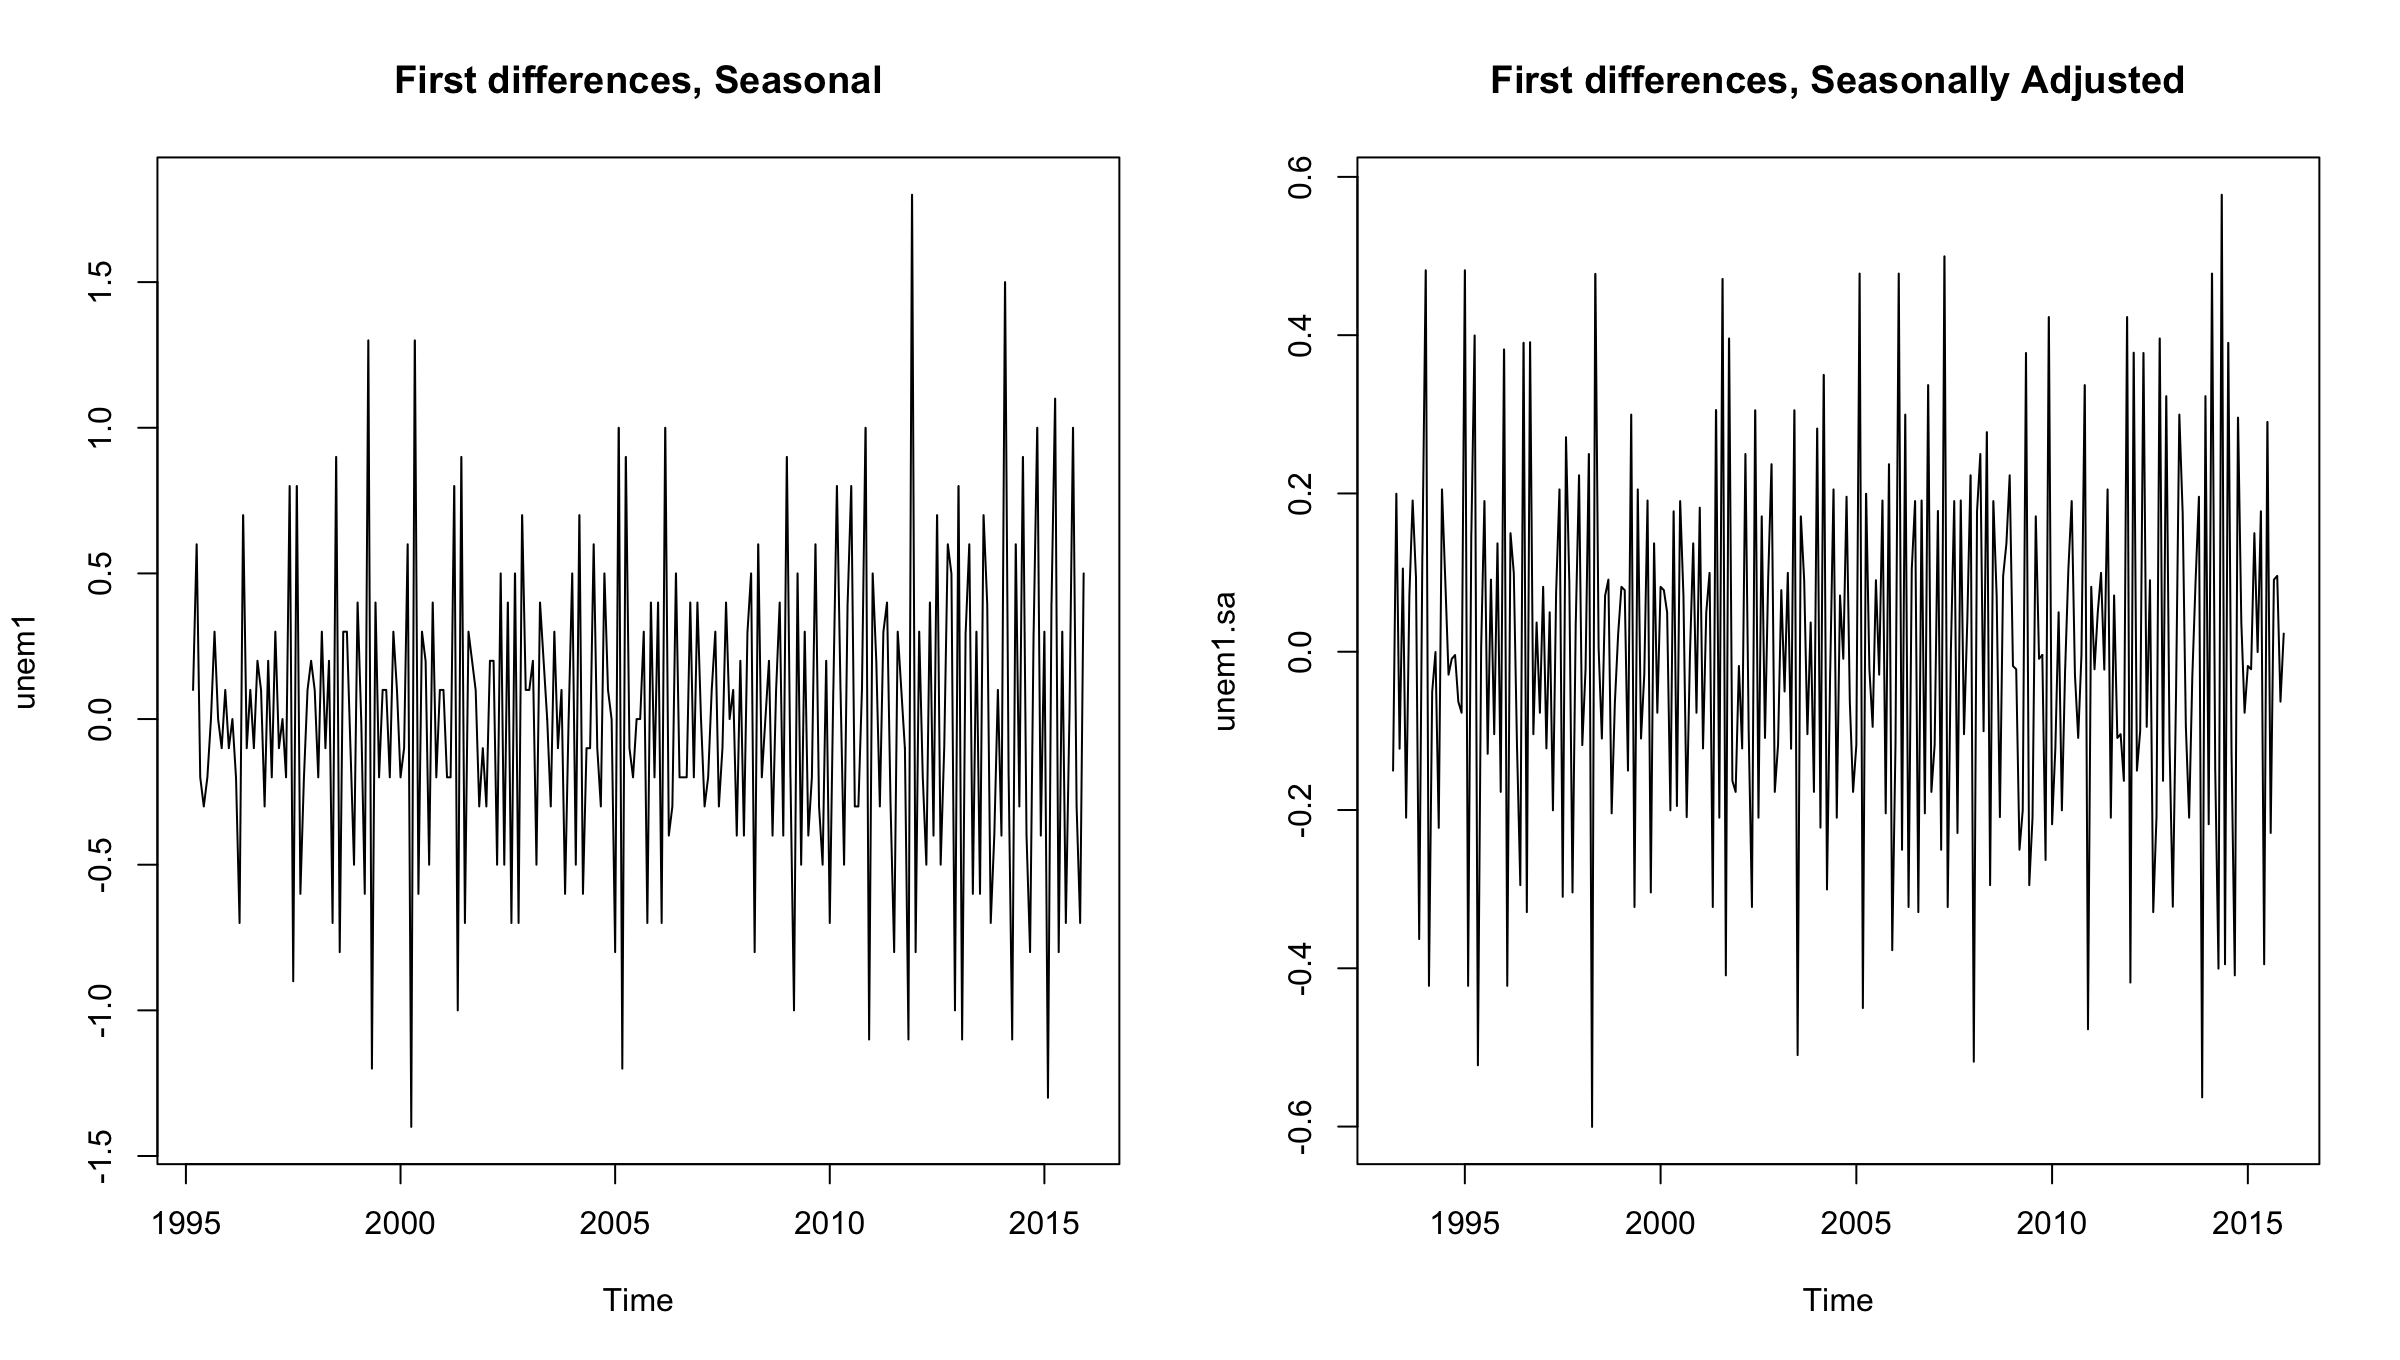
\includegraphics[width=.6\linewidth]{images/firstdiff}
							\caption{Plots of first differences}
							\label{fig:firstdiff}
						\end{figure}
						
								 \begin{figure}[H]
							\centering
							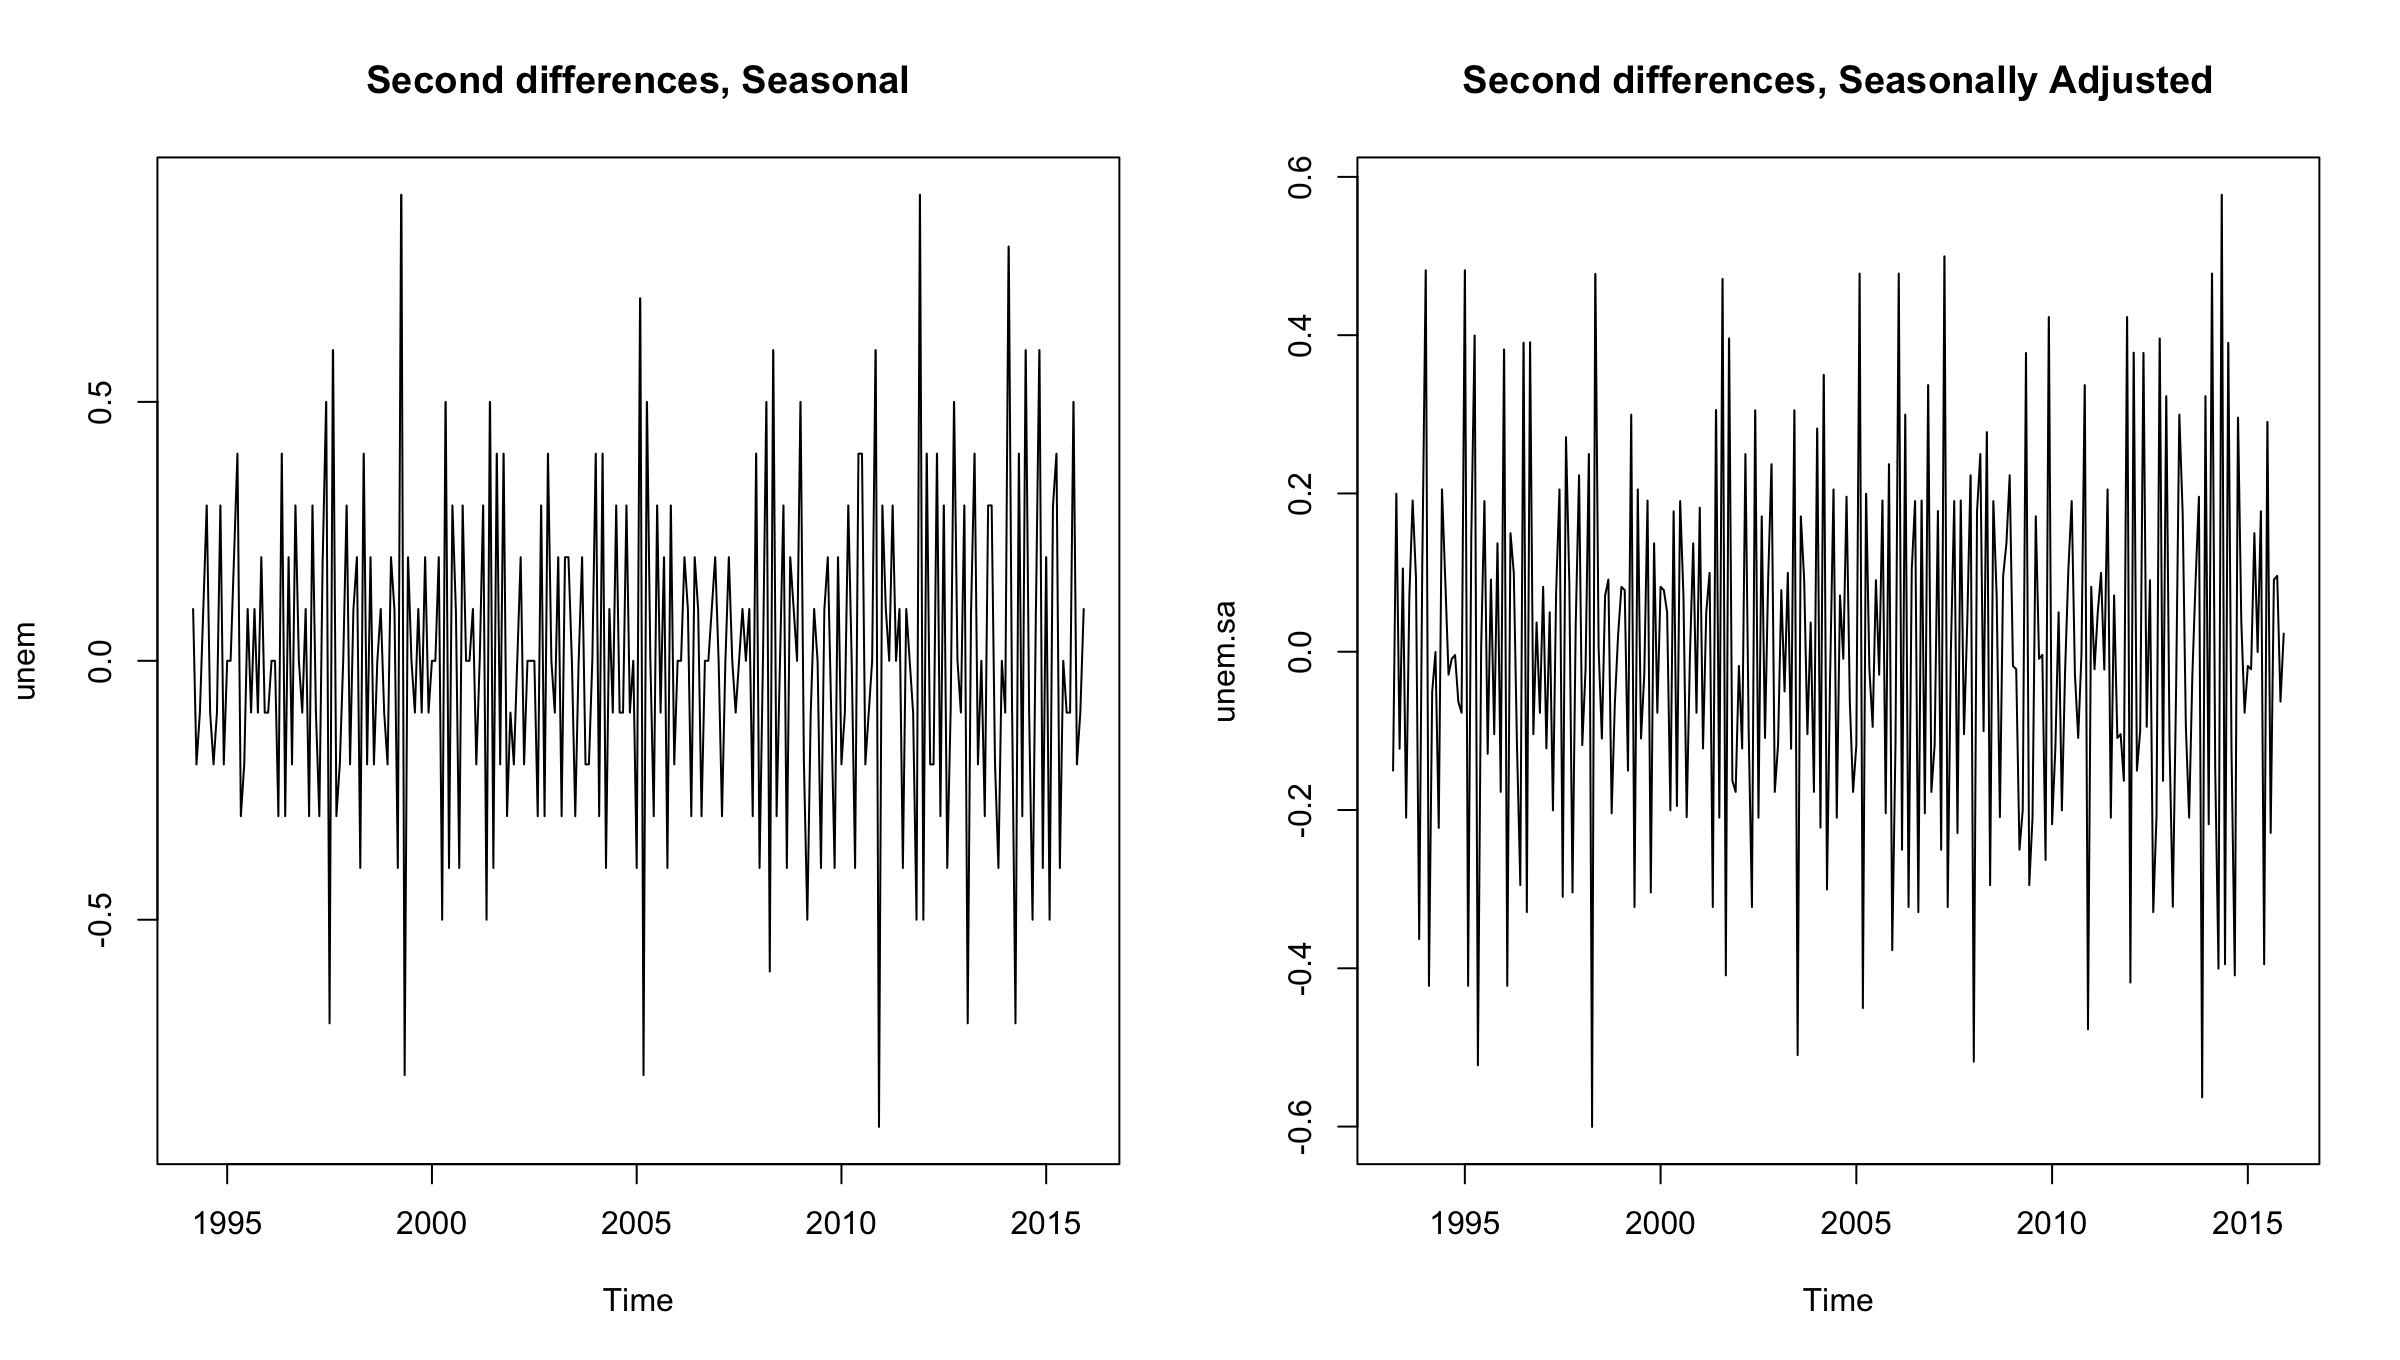
\includegraphics[width=.6\linewidth]{images/secdiff}
							\caption{Plots of second differences}
							\label{fig:secdiff}
						\end{figure}

	 \begin{table}[H]
		 \centering
		 \caption{ADF Test Results}
		 \label{tab:ADF}
		 \begin{tabular}{lllll}
		 \hline
		 \textbf{Model} & \textbf{Statistic} & \textbf{Lag order} & \textbf{p-value}\\ \hline
		 1\(^{st}\) difference &  -7.6799 & 6 & \( < 0.01\)\\
		  1\(^{st}\) difference, SA &  -9.3595 & 6 &\( < 0.01\)\\
		 2\(^{nd}\) difference &  -8.4515 & 6 & \( < 0.01\)\\
		  2\(^{nd}\) difference, SA &  -9.3595 & 6 & \( < 0.01\)\\		 \hline
		 \end{tabular}
		 \end{table}

  
  \subsubsection*{Building the ARIMA \& SARIMA models}
  The team visually analyzed the ACF and PACF plots within the first season (h = 1, 2, ..., 12), see Figure \ref{fig:secdiff2}. The PACF appears to decline slowly, while the ACF seems to fall off after 1. Therefore we began by letting p = 0, and q = 1. Several models were considered by making adjustments to variations resulting in the models found in Table \ref{tab:models}.\newline
  
   \begin{figure}[H]
      	\centering
      	\caption{ACF \& PACF Plots}
      	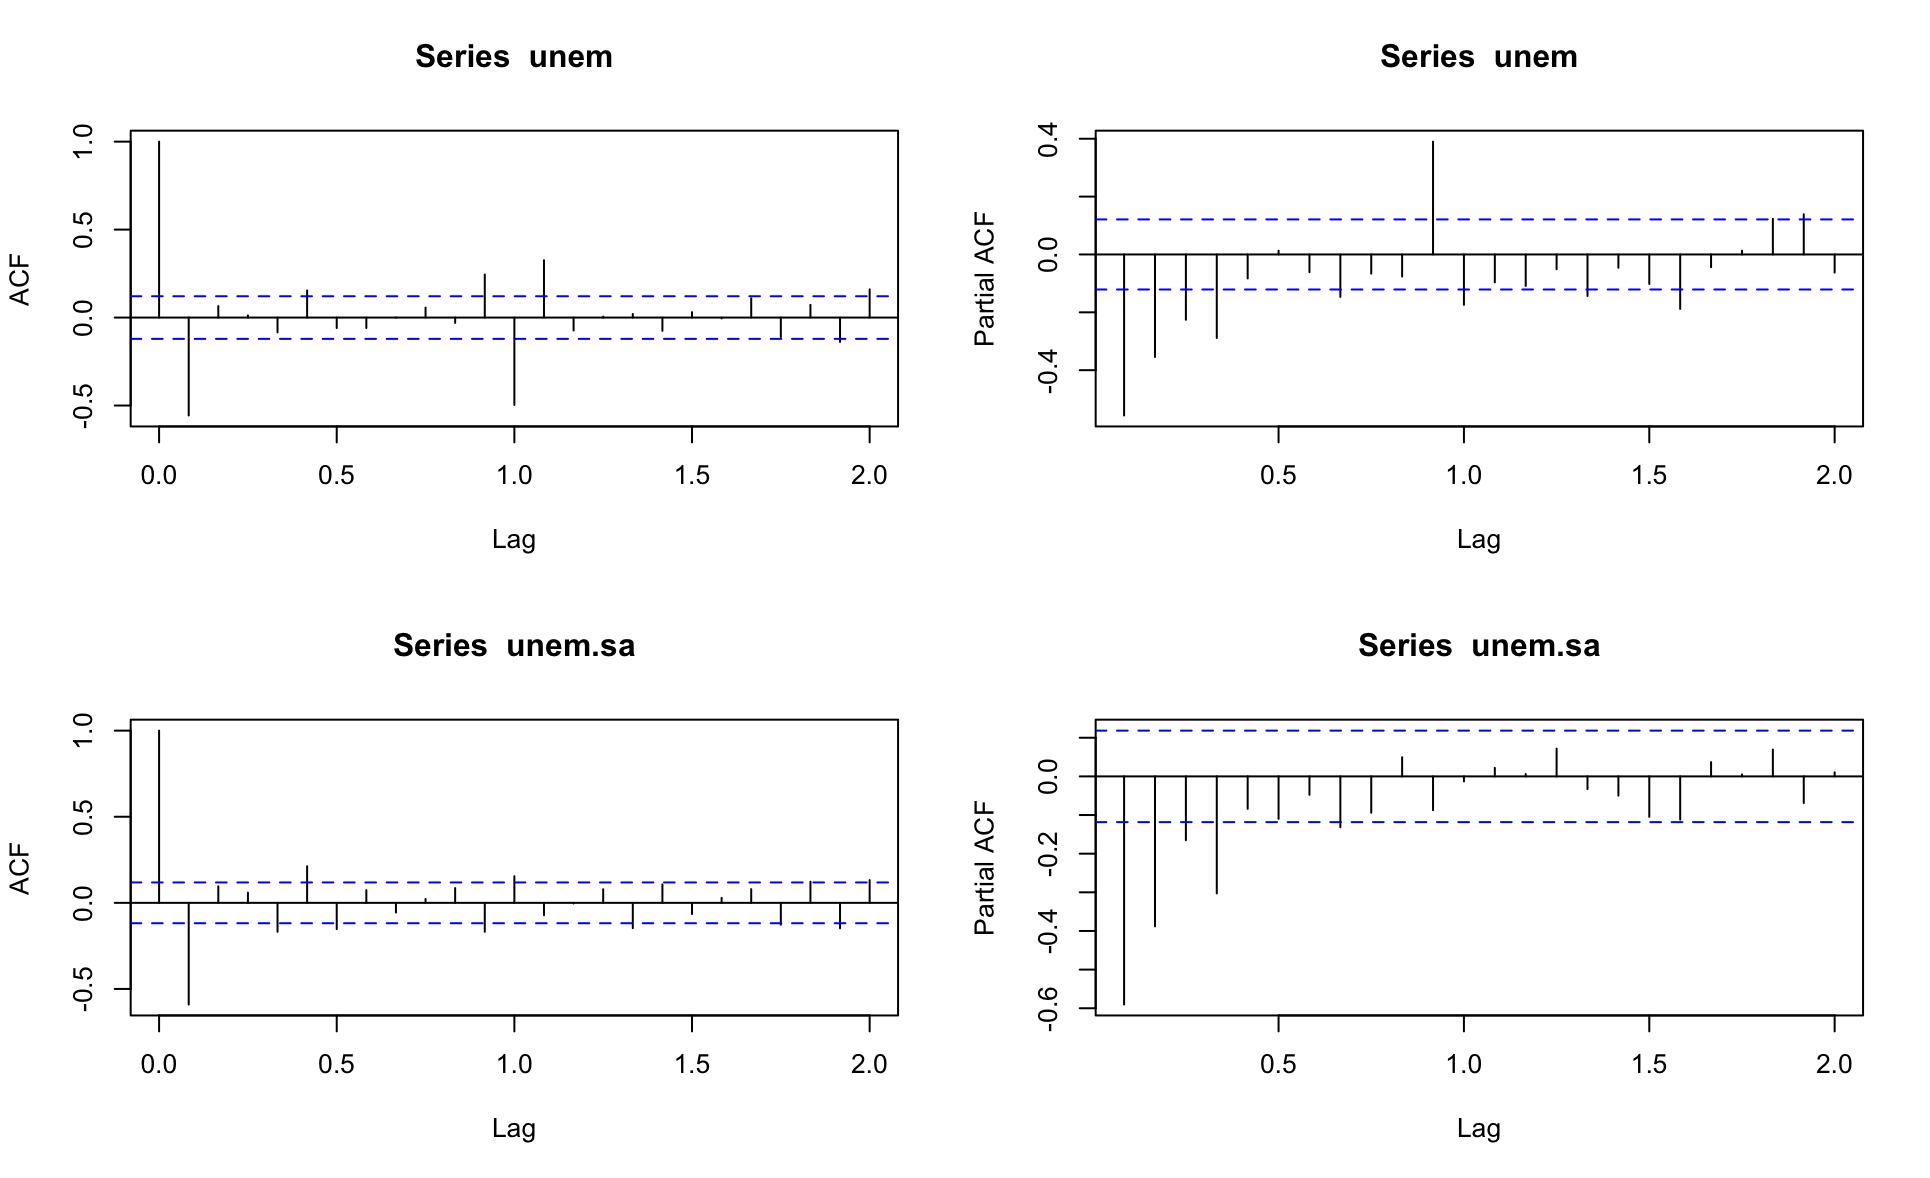
\includegraphics[width=\linewidth]{images/acfpacf}
      	\label{fig:secdiff2}
      \end{figure}
  
     	\begin{table}[H]
     		\centering
     		\caption{Model Summaries}
     		     		\label{tab:models}
     		\begin{tabular}{llccccc}
     			\hline
     			\textbf{\#}& \textbf{Data}  & \textbf{Order} & \textbf{Seasonal} & \textbf{XRegs} & \textbf{AIC} & \textbf{BIC} \\
     			&&&\textbf{Order}&&&\\ 
     			\hline
     			1 & Unem  & 0,2,1 & 1,1,0 & N & -2.27 & -3.23 \\ 
     			2 & Unem  & 0,2,1 & 3,1,0 & N & -2.44 & -3.37 \\ 
     			3 & Unem  & 4,2,1 & 3,1,0 & N & -2.44 & -3.32 \\ 
     			4 & Unem.sa & 0,2,1 & 1,0,0 & N & -2.61 & -3.58 \\ 
     			5 & Unem.sa & 1,2,1 &  & N & -2.63 & -3.60 \\ 
     			6 & Unem.sa & 1,0,1 &  & Y & -2.617 &  -3.578 \\ 
     			7 & Unem.sa & 1,0,1 & & Y& -2.672 &  -3.565\\ \hline
     		\end{tabular}
     	\end{table}

		%-----------------------------------------------------------------------------------------
		
		Based on the AIC values, the two models that show the most promise are models 5 and 7.  Model 5 includes only the time series data whereas model 7 also includes some of the predictors of interest.  The diagnostic plots are shown in Figures \ref{fig:mod5} and \ref{fig:mod7}. Both models show a great deal of promise.  The standardized residuals show no apparent pattern. The ACF of the residuals show no departure from normality. Although the Normal Q-Q plot of the standardized residuals shows some slight departure from normality in the tails, there is no strong evidence of lack of normality in the residuals  The p-values for the  Ljung-Box statistic are high enough at all plotted lags, so there is no indication of lack of fit in the models. Therefore, we will continue to refine these models further as we explore the nature of US Unemployment rate patterns.

\begin{figure}[H]
      	\centering
      	\caption{Model 5 Diagnostics}
      	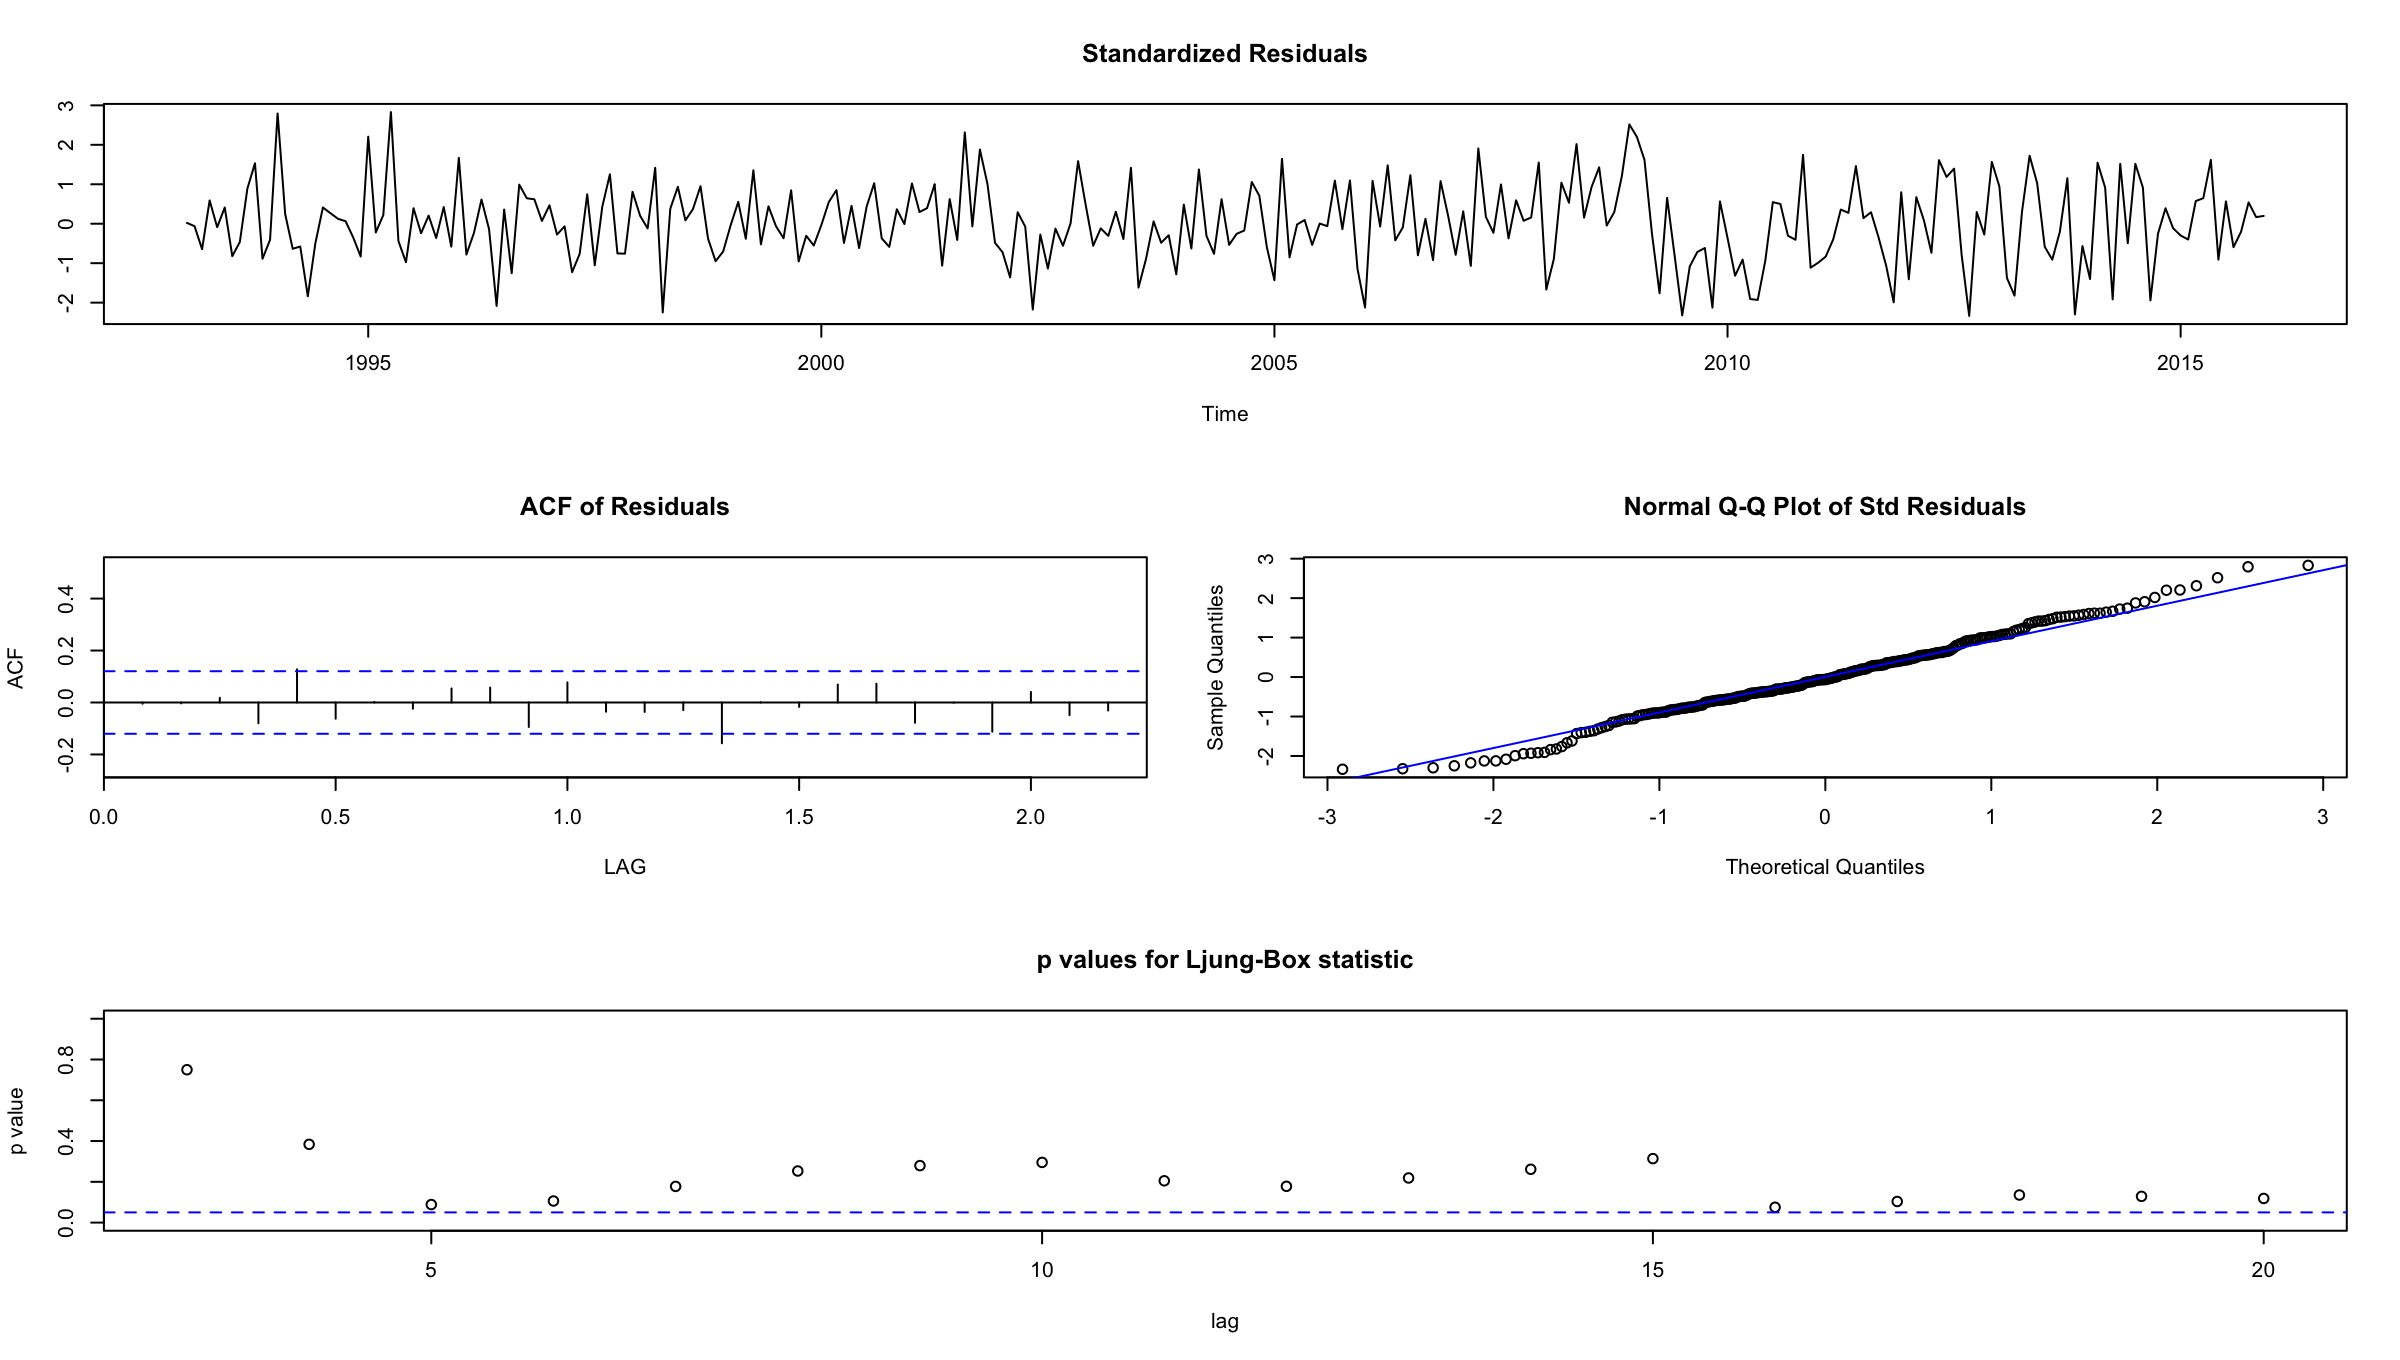
\includegraphics[width=\linewidth]{images/mod5}
      	\label{fig:mod5}
\end{figure}

\begin{figure}[H]
      	\centering
      	\caption{Model 7 Diagnostics}
      	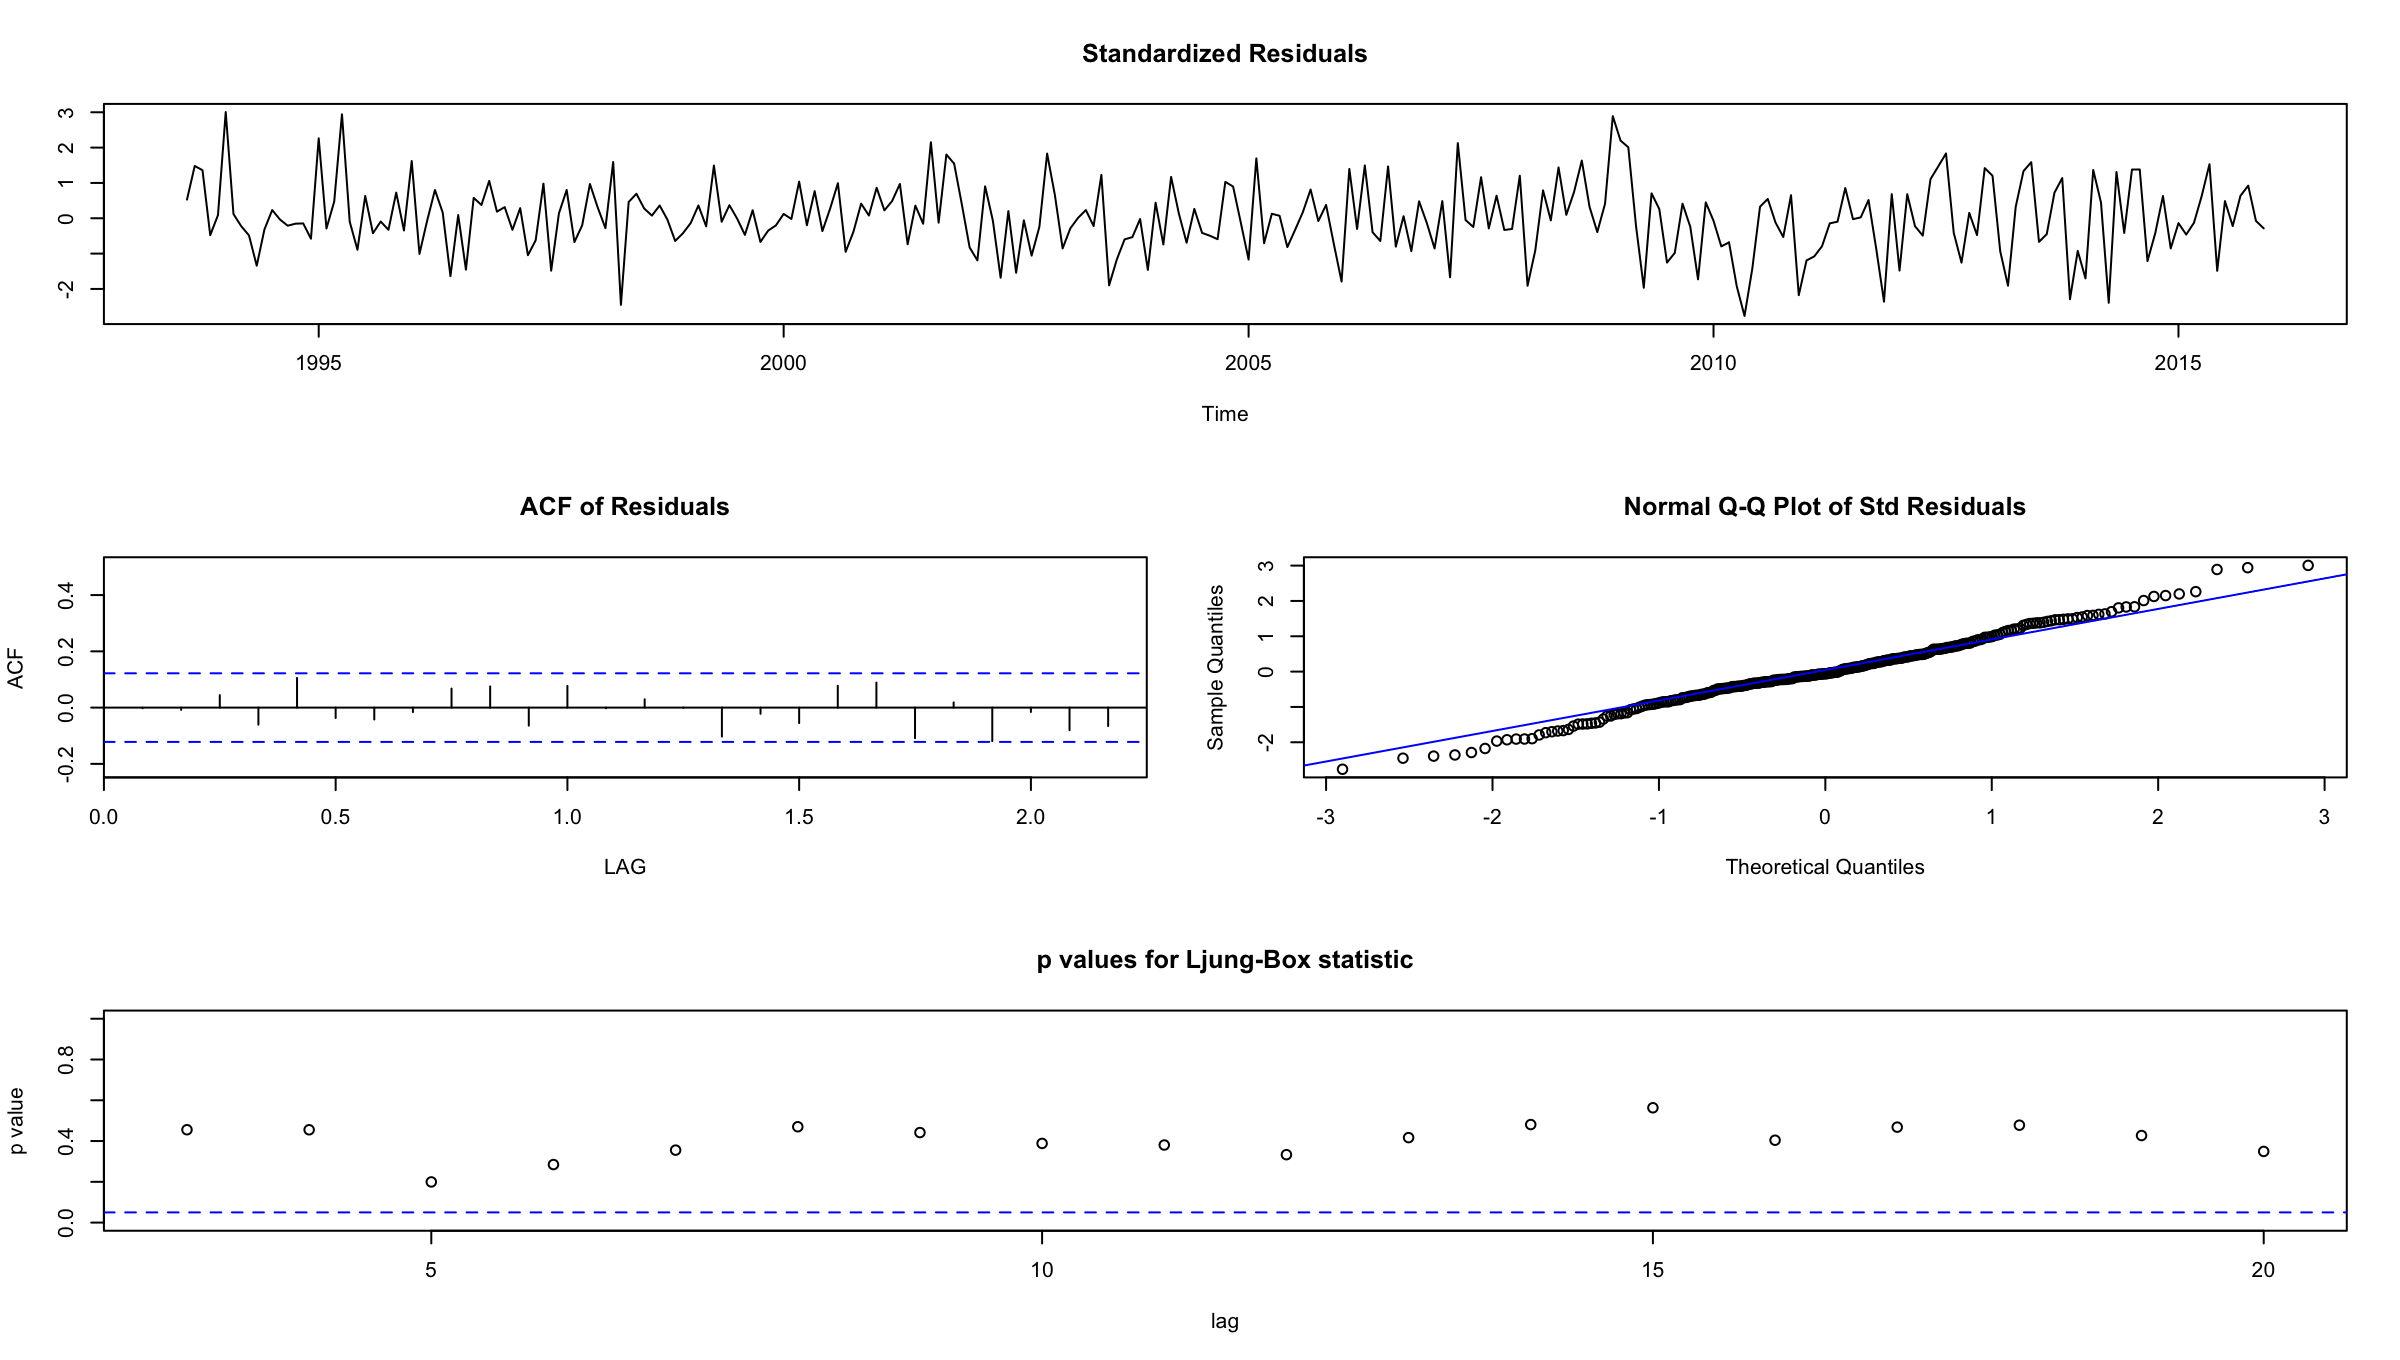
\includegraphics[width=\linewidth]{images/mod7}
      	\label{fig:mod7}
\end{figure}

\bibliographystyle{plainnat} % or try abbrvnat or unsrtnat
\begin{flushleft}
\bibliography{main} % refers to example.bib
\end{flushleft}
}
  

\end{document}